\documentclass[conference]{IEEEtran}
% CSF submission (IEEEtran conference, 2-column). Canonical single-column
% source of truth is ../../main.tex; see NOTES.md for the venue deltas.
\IEEEoverridecommandlockouts

% Essential packages
\usepackage{amsmath,amssymb,amsthm}
\usepackage{mathtools}
\usepackage[numbers,square]{natbib}
\usepackage{booktabs}
\usepackage{graphicx}
\graphicspath{{../../img/}}
\usepackage[hidelinks]{hyperref}
\usepackage{xurl}  % allow long URLs to break, avoiding column overflow
\usepackage{cleveref}
\setlength{\emergencystretch}{3em}  % reduce 2-column prose overfull boxes

% Theorem environments (matching cipher-maps paper)
\theoremstyle{definition}
\newtheorem{definition}{Definition}[section]

\theoremstyle{plain}
\newtheorem{theorem}{Theorem}[section]
\newtheorem{lemma}[theorem]{Lemma}
\newtheorem{corollary}[theorem]{Corollary}
\newtheorem{proposition}[theorem]{Proposition}

\theoremstyle{remark}
\newtheorem{remark}{Remark}[section]
\newtheorem{example}{Example}[section]

% Notation (matching cipher-maps paper)
\newcommand{\fhat}{\hat{f}}
\newcommand{\ghat}{\hat{g}}
\newcommand{\enc}{\mathrm{enc}}
\newcommand{\dec}{\mathrm{dec}}
\newcommand{\im}{\mathrm{Im}}
\newcommand{\TV}{d_{\mathrm{TV}}}
\newcommand{\B}{\{0,1\}}
\DeclareMathOperator{\Uniform}{Uniform}
% Cipher functor: \cipher{X} = C(X) when secret is implicit;
% \cipherS{X}{s} = C_s(X) when secret is explicit.
% Same notation applies to objects (latent types) and morphisms (latent functions).
\newcommand{\cipher}[1]{\mathsf{C}(#1)}
\newcommand{\cipherS}[2]{\mathsf{C}_{#2}(#1)}
\DeclareMathOperator{\orbitF}{orbit}

\title{The Entropy Ratio: Quantitative Confidentiality\\for Trapdoor Computing}
\author{\IEEEauthorblockN{Anonymous Author(s)}\\
\IEEEauthorblockA{Paper submitted for double-blind review}}

\begin{document}

\maketitle

\begin{abstract}
A cipher map is a total function on bit strings implementing a trapdoor
approximation of a latent function: the untrusted machine evaluates it
blindly; only the trusted machine, holding the secret, can encode inputs
and decode outputs.  We develop a quantitative confidentiality theory
for cipher map systems.  The starting point is the entropy ratio
$e = H/H^*$, a normalized form of Shannon leakage borrowed from the
Quantitative Information Flow literature.  We connect this measure to
the cipher map framework's representation-uniformity parameter $\delta$
via the Fannes--Audenaert continuity inequality, giving
$e \geq 1 - \delta - h_2(\delta)/H^*$.  This bridge makes $\delta$ the
operational design target, and we characterize the explicit costs of
the framework's three $\delta$-reduction mechanisms (noise injection,
multiple representations, and encoding granularity), contributing a
Fisher-information dilution result for noise injection.  The paper's
main result is a compositional
leakage theorem with a matching minimax lower bound: even when each
cipher map is marginally $\delta$-uniform, observing multiple
evaluations on a shared cipher value lets the untrusted machine
recover the latent joint distribution to total-variation accuracy
$\xi$ at the \emph{information-theoretically optimal} rate
$\Theta(|Y_1|\cdot|Y_2|/\xi^2)$ (matching upper bound from plug-in
estimation, matching lower bound via Assouad's lemma).  The
compositional channel is therefore not merely exploitable but
unavoidable for any choice of per-cipher-map parameters; reducing
$\delta$ is necessary but not sufficient, and only system-level
interventions (observation limits, joint encoding, or noise
injection) reduce the adversary's effective advantage.  Experimental
validation on encrypted Boolean search over the 20 Newsgroups corpus
confirms the predictions for OR-chain FPR compounding (AND chains
saturate at a construction-level floor) and the encoding granularity
spectrum.
\end{abstract}

\begin{IEEEkeywords}
cipher maps, entropy ratio, Fannes--Audenaert continuity, compositional
leakage, homophonic substitution, quantitative information flow,
trapdoor computing
\end{IEEEkeywords}

%% ====================================================================
\section{Introduction}
\label{sec:intro}
%% ====================================================================

Given a cipher map system---a trusted machine encoding queries, an
untrusted machine evaluating total functions on bit strings, and results
decoded only by the trusted machine---how much does the untrusted machine
learn?

The cipher map framework~\cite{towell2026cipher} provides four properties
(totality, representation uniformity, correctness, composability)
parameterized by $(\eta, \varepsilon, \mu, \delta)$ that characterize
what the untrusted machine can and cannot do.  Totality ensures every
input produces output; representation uniformity bounds frequency
analysis; correctness governs error rates; composability enables chained
evaluation.  But these properties are \emph{qualitative} guarantees.  A
system designer needs \emph{quantitative} answers: given a specific
deployment with a known query distribution, known vocabulary size, and
known resource budget, how confidential is the system, and how can it be
improved?

Confidentiality in cipher map systems
decomposes into two scales.  At the \emph{marginal scale}, a single
cipher map's leakage is controlled by its representation-uniformity
parameter $\delta$, and the per-cipher-value entropy ratio gives a
clean translation.  At the \emph{compositional scale}, observations of
multiple cipher map evaluations on a shared cipher value leak the
joint over latent outputs at parametric rate, independent of $\delta$.
The two scales do not reduce to each other: engineering at one does
not engineer at the other.

That marginal frequency-flattening fails to hide joint structure is,
qualitatively, already known in the encrypted-data setting: multi-column
inference attacks recover correlated columns far beyond what
single-column defenses would suggest~\cite{bindschaedler2018tao}, and
frequency-revealing attacks on frequency-hiding order-preserving
encryption show that hiding a ciphertext marginal leaves joint and
insertion-order structure recoverable~\cite{cao2023frequency}.  Our
contribution is not that observation but its sharp form: we prove the
compositional joint-recovery rate is
$\Theta(|Y_1|\cdot|Y_2|/\xi^2)$ with matching upper and lower bounds,
and that no per-cipher-map parameter, $\delta$ included, lowers this rate.
The structural reason cipher-map confidentiality cannot be reduced to
a single number is therefore a theorem with an information-theoretic
optimality guarantee, not a heuristic observed in attacks, and it is
the spine of the paper.

\paragraph{Marginal scale.}
The central measure is the \emph{entropy ratio} $e = H/H^*$: the ratio
of observed entropy in the cipher map output stream to the maximum
entropy achievable under system constraints.  The measure itself is
not new; it is a normalized form of Shannon leakage studied in the
Quantitative Information Flow literature
(\S\ref{sec:related}).  The cipher map contribution is the connection:
we prove that the representation-uniformity parameter $\delta$
directly lower-bounds the entropy ratio via the Fannes--Audenaert
continuity inequality~\cite{fannes1973continuity,audenaert2007sharp},
\[
e \;\geq\; 1 - \delta - h_2(\delta)/H^*,
\]
where $h_2$ is the binary entropy and $H^* = \log_2|\mathrm{im}(\enc)|$
is the log-size of the populated cipher-value support.  This reduces
marginal-scale
engineering to the concrete problem of minimizing $\delta$.

The cipher map framework provides three mechanisms that reduce
$\delta$.  The cipher maps paper names them and explicitly defers
their cost analysis to this companion
work~\cite[Rem.~5.1]{towell2026cipher}; the \emph{constructions} are
the framework's, and our contribution at the marginal scale is their
analysis as cost-attached levers (the Fisher-information dilution of
the first is the one new mechanism-level result):

\begin{enumerate}
\item \textbf{Noise injection.}  The trusted machine mixes $R$ filler
  queries per $N$ real queries; by totality the untrusted machine
  cannot distinguish real from filler.  Cost: bandwidth ($1 + R/N$).
  Effect: in the bounded-concentration regime, Fisher information for a
  correlation estimator is reduced by $\rho^2 = (N/(N+R))^2$
  (Theorem~\ref{thm:noise-dilution}, new here).

\item \textbf{Multiple representations.}  Each element receives
  $K(x) \geq 1$ encodings, with $K(x) \propto D(x)$ to flatten the
  cipher value distribution (classical homophonic substitution:
  frequent elements get more code symbols so that per-cipher frequency
  equalizes).  The flattening identity is the framework's homophonic
  allocation result~\cite[Prop.~4.1]{towell2026cipher};
  Theorem~\ref{thm:multiplicity} attaches the cost (space:
  $\sum_x K(x)$ slots, with $\delta \to 0$ as the budget grows).

\item \textbf{Encoding granularity}, controlled by an entanglement
  parameter $p$ that interpolates between component-wise encoding
  (correlation leakage) and joint encoding (space $O(|Y|^k)$),
  inherited from~\cite[Sec.~8]{towell2026cipher}.
\end{enumerate}

\paragraph{Compositional scale.}
The constructions above all act at the marginal scale: each cipher map
on its own.  The paper's main result is that this is not enough, and
in a strong sense.  When the untrusted machine observes multiple
cipher map evaluations on a shared cipher value, the joint
distribution over latent outputs is recoverable at the
information-theoretically optimal rate $\Theta(|Y_1|\cdot|Y_2|/\xi^2)$
(matching upper bound from plug-in estimation in
Theorem~\ref{thm:comp-leakage}; matching lower bound via Assouad's
lemma in Theorem~\ref{thm:comp-leakage-lb}); mutual
information is preserved exactly,
$I(\fhat_1(C); \fhat_2(C)) = I(f_1(X); f_2(X))$.  No marginal-scale
parameter, $\delta$ included, changes the rate (Remark~\ref{rem:irreducibility}).
The compositional channel is intrinsic to the framework's
composability, not a bug: the same property that lets the untrusted
machine chain evaluations blindly is the property that creates the
channel.  Defending against a distribution-estimation adversary at
the compositional scale therefore requires system-level interventions
(reducing shared-$c$ observations, joint encoding via
Prop.~\ref{prop:granularity}, or noise injection); marginal-scale
parameter tuning alone does not.  We also include, for completeness,
FPR compounding through Boolean chains, which is inherited
from~\cite[Sec.~7.4]{towell2026cipher}.

\paragraph{Practical measurement.}
We provide practical measurement tools that close the loop between
theory and operation.  The entropy of a cipher map output stream can
be estimated by compressing it: more compressible means more
predictable means less confidential.  This avoids the need for
explicit probabilistic models of the adversary.

\paragraph{Contributions.}
\begin{enumerate}
\item \textbf{Compositional leakage: a rate no per-map parameter can
  move (main result).}  Theorems~\ref{thm:comp-leakage}
  and~\ref{thm:comp-leakage-lb} together establish that no
  per-cipher-map parameter---$\delta$ included, however small---changes
  the rate at which the untrusted machine recovers the latent joint.
  Observing multiple cipher map evaluations on a shared cipher value,
  it reconstructs the joint distribution over latent outputs at the
  information-theoretically optimal rate
  $\Theta(|Y_1|\cdot|Y_2|/\xi^2)$, with mutual-information preservation
  $I(\fhat_1(C); \fhat_2(C)) = I(f_1(X); f_2(X))$.  The upper bound is
  attained by the empirical-distribution plug-in estimator; the
  matching minimax lower bound is via Assouad's lemma.  Reducing
  $\delta$ is therefore necessary but not
  sufficient: only system-level interventions (observation limits,
  joint encoding via Prop.~\ref{prop:granularity}, or noise injection)
  reduce the adversary's effective advantage at this scale.  FPR
  compounding through Boolean chains is included for context; it is
  inherited from~\cite{towell2026cipher} (Appendix~\ref{subsec:fpr-compounding}).

\item \textbf{Fannes bridge.}  The representation-uniformity parameter
  $\delta$ directly lower-bounds the entropy ratio,
  $e \geq 1 - \delta - h_2(\delta)/n$, via the Fannes--Audenaert
  continuity inequality (Theorem~\ref{thm:entropy-decomposition}).
  This makes $\delta$ the operational handle for confidentiality
  engineering in cipher map systems (\S\ref{sec:measure}).

\item \textbf{Cost analysis of the framework's $\delta$-reduction
  levers.}  The cipher maps framework supplies three mechanisms
  (noise injection, multiple representations, encoding granularity) and
  defers their cost analysis to this paper~\cite[Rem.~5.1]{towell2026cipher}.
  We characterize each: noise injection (bandwidth cost $1 + R/N$) with
  a Fisher-information dilution $\rho^2$ that is new here
  (Theorem~\ref{thm:noise-dilution}); multiple representations (space
  cost $\sum_x K(x)$ with $K(x)\propto D(x)$), building on the
  framework's homophonic identity~\cite[Prop.~4.1]{towell2026cipher}
  (Theorem~\ref{thm:multiplicity}); and encoding granularity, used as
  inherited (\S\ref{sec:levers}).

\item \textbf{Practical measurement and validation.}  Compression-based
  entropy estimation avoiding explicit adversary models, and a case
  study demonstrating confidentiality improvement from 72\% to 94\%
  with approximately 1.05$\times$ space and 1.5$\times$ bandwidth
  overhead (Appendix~\ref{sec:measurement},~\S\ref{sec:experiments}).
\end{enumerate}

\paragraph{What this paper does not do.}
We do not use ORAM, FHE, or simulation-based security definitions.
Privacy in the cipher map model comes from the one-way hash, the totality
of $\fhat$, and representation uniformity---not from access-pattern
indistinguishability or computational hardness assumptions beyond the
hash function.  The framework is information-theoretic throughout.


%% ====================================================================
\section{Related Work}
\label{sec:related}
%% ====================================================================

\paragraph{Quantitative information flow.}
The entropy ratio $e = H/H^*$ is a normalized form of Shannon leakage,
studied extensively in the QIF
literature~\cite{smith2009foundations,alvim2020science}.
Smith~\cite{smith2009foundations} proposes min-entropy leakage as a
worst-case measure; Alvim et al.~\cite{alvim2020science} provide a
comprehensive treatment of information-theoretic leakage measures.
The measure itself is not our contribution, and we do not claim
novelty there.  Closer to our compositional result, QIF has studied
how leakage behaves under composition: Kawamoto et
al.~\cite{kawamoto2017compositionality} bound whole-system leakage from
component leakages and observe that, once components are correlated,
the component leakages no longer determine the total; Espinoza and
Smith~\cite{espinoza2012cascade} characterize cascade leakage, and
Smith and Smith~\cite{smith2017tight} give tight bounds on leakage from
repeated independent runs of a channel.  These give \emph{bounds} under
structural assumptions; our compositional theorem
(Theorems~\ref{thm:comp-leakage} and~\ref{thm:comp-leakage-lb}) gives a
\emph{sharp, dimension-dependent rate} $\Theta(|Y_1|\cdot|Y_2|/\xi^2)$
with a matching minimax lower bound, for two distinct maps observed on a
shared cipher value.  The second contribution, the \emph{Fannes bridge}
connecting the representation-uniformity parameter $\delta$ to the
entropy ratio ($e \geq 1 - \delta - h_2(\delta)/n$), makes $\delta$ the
operational handle the QIF measures do not themselves supply.  We
discuss the Shannon-vs-min-entropy choice in \S\ref{sec:discussion}.

\paragraph{Frequency-smoothing and homophonic encryption.}
The marginal-scale lever of \S\ref{sec:levers}---assigning $K(x) \propto
D(x)$ representations per value to flatten the observed cipher-value
distribution---is the classical homophonic substitution of
Simmons~\cite{simmons1979symmetric}, given an information-theoretic
treatment by G{\"u}nther~\cite{gunther1988universal} and Jendal et
al.~\cite{jendal1989information}.  In the encrypted-data setting this
lever is the basis of \emph{frequency-smoothing encryption}: Lacharit{\'e}
and Paterson~\cite{lacharite2018frequency} allocate homophones per record
to defeat snapshot frequency analysis on deterministically encrypted data,
with security stated as game-based indistinguishability and evaluated
empirically for concrete parameters; Chen et
al.~\cite{chen2024revisiting} revisit this line with sharper definitions.
Frequency-hiding order-preserving encryption~\cite{kerschbaum2015frequency}
applies the same multi-ciphertext-per-plaintext idea in the order-preserving
setting, and PANCAKE~\cite{grubbs2020pancake} smooths \emph{access patterns}
to near-uniform with injected fake queries.  Two differences set our
treatment apart.  First, mechanism: representation uniformity is a property
of a \emph{total} cipher map evaluated blindly by the untrusted machine, so
real and filler queries are indistinguishable structurally (by totality)
rather than by an online traffic-injection protocol, and there is no access
stream for a correlation attack to exploit.  Second, and central to this
paper: that line measures the \emph{marginal}---a flattened ciphertext or
access distribution---while the same $\delta$ that flattens the marginal
leaves the joint leakage under composition unbounded.  We prove this gap
as a quantitative separation with a matching minimax rate, which the
frequency-smoothing literature does not contain.

\paragraph{Multi-field and correlated inference.}
The compositional phenomenon---marginal hiding leaving the joint
recoverable---has been observed and attacked, though not given a matching
rate.  Bindschaedler et al.~\cite{bindschaedler2018tao} give an
analytically optimal multinomial inference attack that, extended across
correlated columns, recovers far more than single-column defenses suggest;
Cao et al.~\cite{cao2023frequency} show frequency-hiding order-preserving
encryption leaks recoverable joint and insertion-order structure despite a
hidden marginal; and the leakage-abuse line~\cite{cash2015leakage,
naveed2015inference,islam2012access} demonstrates inference from preserved
or co-occurrence structure.  Our Theorems~\ref{thm:comp-leakage}
and~\ref{thm:comp-leakage-lb} supply what these attacks observe but do not
prove: the information-theoretically optimal rate of joint recovery and its
irreducibility by any per-map parameter.  The empirical evaluation
frameworks for such attacks~\cite{kamara2022sok} are complementary; we give
the analytic rate, and use the 20 Newsgroups corpus
(\S\ref{sec:experiments}) to validate it.

\paragraph{SSE leakage mitigation.}
Noise injection for encrypted search has been studied in the SSE
literature.
Bost and Fouque~\cite{bost2017thwarting} propose dummy queries with
game-based security analysis; Demertzis et al.~\cite{demertzis2020seal}
develop tunable leakage-functionality trade-offs.
Our analysis differs in using information-theoretic measures (entropy
ratio) rather than simulation-based definitions, and applies to general
cipher maps, not only encrypted search.

\paragraph{Leakage from property-preserving encryption.}
Naveed et al.~\cite{naveed2015inference} and Islam et
al.~\cite{islam2012access} demonstrate inference attacks exploiting
preserved algebraic structure.
The cipher map model avoids property preservation entirely: the untrusted
machine evaluates a total function on opaque bit strings and cannot
determine the output type from the cipher value.

%% ====================================================================
\section{Preliminaries}
\label{sec:prelim}
%% ====================================================================

We recall the cipher map abstraction from~\cite{towell2026cipher}.  All
notation follows that paper; we cite rather than re-derive.

\begin{definition}[Cipher map~{\cite[Def.~3.1]{towell2026cipher}}]
\label{def:cipher-map}
A \emph{cipher map} for a latent function $f : X \to Y$ is a tuple
$(\fhat, \enc, \dec, s)$ where $\fhat : \B^n \to \B^n$ is a total
function on $n$-bit strings, $\enc : X \times \{0,\ldots,K(x){-}1\}
\to \B^n$ is an encoding function with $K(x) \geq 1$ representations
per element, $\dec : \B^n \to Y \cup \{\bot\}$ is a decoding function,
and $s$ is a secret (the trapdoor).  The untrusted machine holds $\fhat$.
The trusted machine holds $\enc$, $\dec$, and $s$.
\end{definition}

The four properties, parameterized by
$(\eta, \varepsilon, \mu, \delta)$~\cite[Sec.~4]{towell2026cipher}:

\begin{description}
\item[Totality.]  $\fhat$ is defined on all $2^n$ inputs.  Out-of-domain
  outputs are indistinguishable from uniform under the random oracle
  model.

\item[Representation uniformity ($\delta$-bounded).]  The marginal
  distribution $Q$ of cipher values is $\delta$-close to uniform over the
  \emph{image} $\mathrm{im}(\enc)$ in total variation:
  $\TV(Q, U_{\mathrm{im}}) = \frac{1}{2}\sum_c |Q(c) - U_{\mathrm{im}}(c)|
  \leq \delta$.  (The image, not the ambient $\B^n$: a sparse-image
  construction has $\TV(Q, U_{\B^n}) \approx 1$ trivially, so the
  meaningful uniformity is relative to the support the trusted machine
  populates.  Under the random oracle model $\mathrm{im}(\enc)$ is
  pseudorandom in $\B^n$, so an adversary that cannot locate the image
  inherits the same bound against ambient uniform up to a birthday term;
  see Theorem~\ref{thm:multiplicity}.)  Informally, $\delta$ bounds the
  advantage of a frequency test trying to distinguish real cipher values
  from uniform ones on the populated support.

\item[Correctness ($\eta$-bounded).]  The fraction of domain elements
  that decode incorrectly is at most $\eta$:
  \[
  \Pr[\dec(\fhat(\enc(x,k))) \neq f(x)] \leq \eta.
  \]
  Nonzero $\eta$ provides plausible deniability (an observed result might
  be wrong) and reduces construction cost.

\item[Noise-decode probability ($\varepsilon$).]  A random $n$-bit
  string decodes to a valid output with probability $\varepsilon$.
  Lower $\varepsilon$ means out-of-domain queries are more likely to be
  rejected (decoded as $\bot$), at the cost of more bits per element.

\item[Value cost ($\mu = H(Y)$).]  The average number of bits needed to
  encode one output value, equal to the Shannon entropy of the output
  distribution.

\item[Composability.]  The composition of two cipher maps is again a
  cipher map: $\ghat \circ \fhat$ has correctness
  $\eta_{g \circ f} \leq 1 - (1 - \eta_f)(1 - \eta_g)$.
  Errors accumulate predictably, enabling pipeline analysis.
\end{description}

The space per element decomposes as
$\text{bits/element} = -\log_2 \varepsilon + H(Y)$, where
$-\log_2 \varepsilon$ bits distinguish signal from noise and
$H(Y) = \mu$ bits encode the function
value~\cite[Thm.~6.1]{towell2026cipher}.

\paragraph{Trusted/untrusted model.}
The trusted machine $T$ encodes inputs, decodes results, and injects
filler queries.  The untrusted machine $U$ evaluates $\fhat$ on any bit
string and returns results.  $U$ cannot decode, distinguish real from
filler queries, determine the domain $X$, or enumerate which inputs are
``in-domain''~\cite[Sec.~5]{towell2026cipher}.

\paragraph{Acceptance predicates.}
The batch construction of a cipher map is unified under an
\emph{acceptance predicate}: a family of disjoint sets
$\{A(y) \subseteq \B^n : y \in Y\}$ that partitions hash space among
output values~\cite[Sec.~6.2]{towell2026cipher}.  Shannon-optimal
allocation sets $|A(y)| \propto \Pr[f(X) = y]$, simultaneously
minimizing space and maximizing output indistinguishability.

\paragraph{Information-theoretic notation.}
We use standard information-theoretic quantities throughout.
\emph{Shannon entropy} $H(X) = -\sum_x p(x) \log_2 p(x)$ measures the
average surprise (in bits) of a random variable; higher entropy means
less predictable.
\emph{Conditional entropy} $H(X \mid Y)$ is the remaining uncertainty in
$X$ after observing $Y$.
\emph{Mutual information} $I(X; Y) = H(X) - H(X \mid Y)$ quantifies how
much observing $Y$ reveals about $X$; zero means independence.
\emph{KL divergence} $D_{\mathrm{KL}}(P \| Q) = \sum_x P(x) \log_2
(P(x)/Q(x))$ measures how far $P$ is from $Q$; it is zero iff $P = Q$
and connects to the entropy ratio via $H(P) = H^* - D_{\mathrm{KL}}(P
\| U)$ when $U$ is the maximum-entropy (uniform) distribution.
We use $D$ for the distribution of queries over the domain $X$, and $Q$
for the induced distribution over cipher values.
All logarithms are base~2.


%% ====================================================================
\section{The Confidentiality Measure}
\label{sec:measure}
%% ====================================================================

This section and~\S\ref{sec:levers} develop the marginal-scale theory
introduced in~\S\ref{sec:intro}: how to measure single-cipher-map
leakage via the entropy ratio, and how to engineer toward the design
target $\delta$.  The compositional-scale theory is in~\S\ref{sec:composition}.

\subsection{Observed and Maximum Entropy}

Consider a cipher map system in which the trusted machine submits a
stream of cipher values to the untrusted machine.  The untrusted machine
observes a sequence $c_1, c_2, \ldots, c_N$ of $n$-bit strings, each
either a real encoding $\enc(x_i, k_i)$ or a filler string drawn
uniformly from $\B^n$.

\begin{definition}[Observed entropy]
\label{def:observed-entropy}
The \emph{observed entropy} $H$ of a cipher map system is the Shannon
entropy of the joint distribution over the observable sequence:
\begin{equation}
H = H(C_1, C_2, \ldots, C_N),
\end{equation}
where each $C_i$ is the random variable corresponding to the $i$-th
cipher value observed by the untrusted machine.
\end{definition}

\begin{definition}[Maximum entropy under constraints]
\label{def:max-entropy}
The \emph{maximum entropy} $H^*$ is the maximum of $H$ over all
distributions on the observable sequence that are consistent with the
system constraints: domain size $|X|$, codomain size $|Y|$, and the
cipher map parameters $(\eta, \varepsilon, \delta)$.
\end{definition}

By the maximum entropy principle~\cite{jaynes1957information}, $H^*$ is
achieved when the observable distributions are as uniform as possible
subject to the constraints.  For a single cipher value drawn from a
vocabulary of size $m$, the maximum entropy is $\log_2 m$ (uniform
distribution).  For a sequence of $N$ independent cipher values, the
maximum entropy is $N \log_2 m$.

\subsection{The Entropy Ratio}

\begin{definition}[Entropy ratio]
\label{def:entropy-ratio}
The \emph{entropy ratio} of a cipher map system is
\begin{equation}
\label{eq:entropy-ratio}
e = \frac{H}{H^*} \in [0, 1].
\end{equation}
\end{definition}

The entropy ratio has a direct operational interpretation:

\begin{itemize}
\item $e = 0$: the output sequence is fully predictable.  The untrusted
  machine can predict every cipher value with certainty.  No
  confidentiality.

\item $e = 1$: the output sequence is indistinguishable from the maximum
  entropy distribution under system constraints.  The untrusted machine's
  best prediction is no better than guessing from the maximum entropy
  distribution.  Maximum confidentiality.
\end{itemize}

\subsection{Relationship to Cipher Map Parameters}

The entropy ratio connects to the four cipher map parameters through the
following result.

\begin{theorem}[Entropy ratio decomposition]
\label{thm:entropy-decomposition}
Let $(\fhat, \enc, \dec, s)$ be a cipher map for $f : X \to Y$ with
parameters $(\eta, \varepsilon, \mu, \delta)$.  Let $D$ be the query
distribution on $X$, and let $Q$ be the induced distribution on cipher
values.  Then the per-query observed entropy satisfies:
\begin{equation}
\label{eq:entropy-decomp}
H(Q) = H^* - D_{\mathrm{KL}}(Q \| U)
      = H^* \!\left(1 - \frac{D_{\mathrm{KL}}(Q \| U)}{H^*}\right),
\end{equation}
where $U$ is the uniform distribution on $\B^n$ and the entropy ratio is
$e = H(Q)/H^* = 1 - D_{\mathrm{KL}}(Q \| U)/H^*$.  In particular:
\begin{enumerate}
\item If $\delta = 0$ (perfect representation uniformity), then
  $Q = U_{\mathrm{im}}$ and $H(Q) = H^* = \log_2|\mathrm{im}(\enc)|$,
  giving $e = 1$.
\item If $K(x) = 1$ for all $x$ (simple substitution, no multiple
  representations), then $\enc$ is injective, $\mathrm{im}(\enc)$ has
  $|X|$ elements, and $Q$ is a relabeling of $D$, so
  $e = H(D) / \log_2 |X|$.
\item For $\delta \leq 1/2$, the entropy ratio is bounded by
  \[
  e \geq 1 - \delta - h_2(\delta)/H^*,
  \qquad H^* = \log_2|\mathrm{im}(\enc)|,
  \]
  where $h_2(\delta) = -\delta\log_2\delta - (1-\delta)\log_2(1-\delta)$
  is the binary entropy.  The bound follows from the Fannes--Audenaert
  continuity inequality~\cite{fannes1973continuity,audenaert2007sharp}
  applied on the image.
\end{enumerate}
\end{theorem}

\begin{proof}
For part (1): when $\delta = 0$, $Q$ is uniform over $\B^n$ by
definition of representation uniformity.  The entropy of the uniform
distribution on $2^n$ elements is $n$ bits, which equals $H^*$.

For part (2): with $K(x) = 1$, the encoding $\enc$ is injective, so $Q$
is a relabeling of $D$.  Entropy is invariant under bijection, giving
$H(Q) = H(D)$.  The maximum over distributions on $|X|$ elements is
$\log_2 |X|$, so $e = H(D) / \log_2 |X|$.

For part (3): the Fannes--Audenaert inequality bounds entropy
continuity: for any distributions $P, Q$ on a support of size $d$ with
$\TV(P, Q) \leq t \leq 1/2$,
\[
|H(P) - H(Q)| \;\leq\; t \log_2(d - 1) + h_2(t).
\]
Applying this to $Q$ and $U_{\mathrm{im}}$ on $\mathrm{im}(\enc)$ with
$d = |\mathrm{im}(\enc)|$, $H^* = \log_2 d$, and
$\TV(Q, U_{\mathrm{im}}) \leq \delta$,
\[
|H(Q) - H^*| \;\leq\; \delta \log_2(d - 1) + h_2(\delta)
                \;\leq\; \delta H^* + h_2(\delta),
\]
so $H(Q) \geq H^*(1 - \delta) - h_2(\delta)$ and
$e = H(Q)/H^* \geq 1 - \delta - h_2(\delta)/H^*$.
Note the bound is linear in $\delta$ (not quadratic):
Pinsker gives $D_{\mathrm{KL}} \geq 2\,\TV^2$, an upper bound on TV
given KL, which does not convert to a KL bound given TV.  The correct
direction is Fannes--Audenaert.
\end{proof}

\begin{remark}[Which support normalizes $H^*$]
\label{rem:hstar}
The maximum entropy $H^*$ is the log-size of the cipher-value support the
construction actually populates, $H^* = \log_2|\mathrm{im}(\enc)|$: the
entropy ratio measures how close the observed marginal is to uniform
\emph{on that support}, the only uniformity a sparse-image construction
can achieve (ambient uniform over all of $\B^n$ sits at TV distance
$\approx 1 - |\mathrm{im}(\enc)|/2^n \approx 1$ from any such $Q$, hence
is useless as a target).  For a simple substitution (part 2) the image
has $|X|$ elements, so $H^* = \log_2|X|$.  Under the random oracle model
the image is pseudorandom in $\B^n$, so a computationally bounded
adversary that cannot locate it sees the same bound against ambient
uniform up to a birthday term (Theorem~\ref{thm:multiplicity}); that
ambient view is the cryptographic layer, while
$H^* = \log_2|\mathrm{im}(\enc)|$ is the information-theoretic measure
used throughout, including the examples and case study of
\S\ref{sec:levers} and~\S\ref{sec:experiments}.
\end{remark}

\begin{remark}[Numerical scale]
For a populated support of $H^* = 32$ bits and $\delta = 0.05$, the bound
gives $e \geq 1 - 0.05 - h_2(0.05)/32 \approx 0.941$; for $\delta = 0.01$,
$e \geq 0.987$.  The $h_2(\delta)/H^*$ correction is negligible once the
support exceeds a few thousand values, so the bound is effectively
linear, $e \gtrsim 1 - \delta$: tightening $\delta$ by an order of
magnitude tightens the leakage bound by roughly the same order.
\end{remark}

\begin{remark}[The role of $\varepsilon$]
The noise decode probability $\varepsilon$ does not appear directly in
the per-query entropy, but it determines the space cost: achieving small
$\varepsilon$ requires $-\log_2 \varepsilon$ bits per element.  The
indirect effect is that larger $\varepsilon$ means a denser cipher space
(more random bit strings decode to valid outputs), which helps uniformity
but increases false positives.
\end{remark}

\begin{remark}[The role of $\eta$]
The correctness parameter $\eta$ provides a form of plausible
deniability.  With $\eta > 0$, the untrusted machine cannot be certain
that a decoded output reflects the true function value.  This adds
$H_b(\eta) = -\eta \log_2 \eta - (1-\eta) \log_2(1-\eta)$ bits of
uncertainty per query (the binary entropy of the error event).
\end{remark}


%% ====================================================================
\section{Constructions for Reducing \texorpdfstring{$\delta$}{delta}}
\label{sec:levers}
%% ====================================================================

The cipher map framework supplies three mechanisms that reduce
$\delta$ (\S\ref{sec:intro}); this section analyzes each as a
cost-attached lever.  The constructions are the framework's; the cost
characterizations, and the Fisher-information dilution of noise
injection (\S\ref{subsec:noise}), are this paper's marginal-scale
contribution.

\subsection{Noise Injection}
\label{subsec:noise}

The trusted machine can mix $R$ filler queries with $N$ real queries.  By
totality, the untrusted machine cannot distinguish real from filler: both
are $n$-bit strings, and $\fhat$ produces $n$-bit output on both.

\begin{theorem}[Noise dilution]
\label{thm:noise-dilution}
Assume $K(x) = 1$ (single encoding per element), so the cipher value
distribution of real queries equals $D$.
Let the trusted machine submit $N$ real queries drawn from $D$ and
$R$ filler queries drawn uniformly from the image $\mathrm{im}(\enc)$,
the populated cipher-value support (the trusted machine samples it
directly; ambient-uniform filler over all of $\B^n$ is indistinguishable
from a single real observation under the random oracle model but is
separable from real queries by repetition frequency over a stream, so we
draw filler from the support real queries actually occupy).  The mixed
sequence has $N + R$ elements, each of which is real with probability
$\rho = N / (N + R)$ and filler with probability $1 - \rho$.  Write
$U_{\mathrm{im}}$ for the uniform distribution on $\mathrm{im}(\enc)$ and
$H^* = \log_2|\mathrm{im}(\enc)|$.  Then:
\begin{enumerate}
\item The observed per-element distribution is the mixture
  $Q_{\mathrm{mix}} = \rho\,D + (1 - \rho)\,U_{\mathrm{im}}$, whose
  entropy obeys
\begin{equation}
\label{eq:noise-entropy}
\begin{aligned}
H_{\mathrm{mix}} &\geq \rho\,H(D) + (1 - \rho)\,H^*,\\
H_{\mathrm{mix}} &\leq \rho\,H(D) + (1 - \rho)\,H^* + H_b(\rho),
\end{aligned}
\end{equation}
where $H_b(\rho)$ is the binary entropy of $\rho$ and the upper bound is
attained only when the real and filler supports are disjoint.  Because
real and filler both live on $\mathrm{im}(\enc)$ the inequality is
strict: the naive sum on the right over-counts by the indicator entropy
$H(B \mid Q_{\mathrm{mix}})$, where $B$ is the real/filler label the
untrusted machine never observes.

\item As $R/N \to \infty$, $Q_{\mathrm{mix}} \to U_{\mathrm{im}}$, so
  $H_{\mathrm{mix}} \to H^*$ and $e \to 1$.

\item For any one-dimensional parameter $\theta$ of $D$, the
  Fisher information satisfies
  \begin{equation}
  \label{eq:fisher-noise}
  I^{\mathrm{mix}}(\theta) \;\leq\; \rho^2 \cdot C(D) \cdot I^{\mathrm{pure}}(\theta),
  \end{equation}
  where $I^{\mathrm{pure}}(\theta)$ is the Fisher information from
  observing $D$ directly and
  $C(D) = \max_c D(c) / U_{\mathrm{im}}(c) = |\mathrm{im}(\enc)| \max_c D(c)$
  is the worst-case concentration of $D$ relative to uniform on the
  image.  The $\rho^2$ dilution is operative only when $C(D) = O(1)$
  (i.e.\ $D$ within a bounded ratio of uniform on its support), which
  requires $\rho \lesssim 1/\sqrt{C(D)}$ for $\rho^2 C(D) < 1$ to make
  the bound a genuine reduction; in that regime the variance of any
  unbiased estimator scales as
  $\Omega\!\bigl((1 + R/N)^2 / C(D)\bigr) \cdot \mathrm{Var}_{\mathrm{pure}}$.
  For heavily concentrated $D$ ($C(D) \gg 1$) the heavy elements stay
  individually identifiable, so noise injection raises the marginal
  entropy ratio (part 1) without diluting correlation estimation.
\end{enumerate}
\end{theorem}

\begin{proof}
For part (1): the observed value has distribution
$Q_{\mathrm{mix}} = \rho D + (1-\rho) U_{\mathrm{im}}$ directly.  Let
$B \in \{\text{real},\text{filler}\}$ be the unobserved source indicator,
so $H(B) = H_b(\rho)$ and
$H(Q_{\mathrm{mix}} \mid B) = \rho H(D) + (1-\rho) H^*$.  The chain rule
gives $H(Q_{\mathrm{mix}}, B) = H_b(\rho) + \rho H(D) + (1-\rho) H^*$.
The untrusted machine observes $Q_{\mathrm{mix}}$ but not $B$, so its
entropy is $H_{\mathrm{mix}} = H(Q_{\mathrm{mix}}) = H(Q_{\mathrm{mix}}, B)
- H(B \mid Q_{\mathrm{mix}}) \leq H_b(\rho) + \rho H(D) + (1-\rho) H^*$,
with equality iff $B$ is a function of $Q_{\mathrm{mix}}$ (disjoint
supports).  Concavity of entropy gives the matching lower bound
$H_{\mathrm{mix}} \geq \rho H(D) + (1-\rho) H^*$.

For part (2): as $\rho \to 0$, $Q_{\mathrm{mix}} \to U_{\mathrm{im}}$ and
$H_{\mathrm{mix}} \to H^*$.

For part (3): write the mixture density at observation $c$ as
$P_{\mathrm{mix}}(c \mid \theta) = \rho P_\theta(c) +
(1 - \rho) U_{\mathrm{im}}(c)$.  The score is
$\partial_\theta \log P_{\mathrm{mix}} =
\rho\,\partial_\theta P_\theta / P_{\mathrm{mix}}$, so
\[
I^{\mathrm{mix}}(\theta)
  = \mathbb{E}_{\mathrm{mix}}\!\left[\bigl(\partial_\theta \log P_{\mathrm{mix}}\bigr)^2\right]
  = \rho^2 \int \frac{(\partial_\theta P_\theta)^2}{P_{\mathrm{mix}}}\,dc.
\]
The pointwise inequality $P_\theta(c) \leq C(D)\,P_{\mathrm{mix}}(c)$
holds because $C(D)\,P_{\mathrm{mix}}(c) \geq (1-\rho)\,C(D)\,
U_{\mathrm{im}}(c) = (1-\rho)\max_{c'} P_\theta(c') \geq (1-\rho)
P_\theta(c)$ while the real term contributes
$\rho\,C(D)\,P_\theta(c) \geq \rho P_\theta(c)$, and these sum to
$P_\theta(c)$.  Hence $1/P_{\mathrm{mix}}(c) \leq C(D)/P_\theta(c)$ and
\[
I^{\mathrm{mix}}(\theta)
  \leq \rho^2\,C(D) \int \frac{(\partial_\theta P_\theta)^2}{P_\theta}\,dc
  = \rho^2\,C(D)\,I^{\mathrm{pure}}(\theta),
\]
with $C(D) = \max_c P_\theta(c) / U_{\mathrm{im}}(c) =
|\mathrm{im}(\enc)| \max_c P_\theta(c)$.  The Cram\'er--Rao bound gives
the variance claim.  $C(D)$ is unbounded as $D$ concentrates, so the
$\rho^2$ reduction is operative only for $D$ of bounded ratio to uniform
on its support (the regime condition in the statement).
\end{proof}

\begin{remark}[Relation to Fisher-information privacy]
Using Fisher information as a privacy measure---certifying a mechanism by
how much it lowers the Fisher information available to any estimator, via
the Cram\'er--Rao bound---is the approach of Farokhi and
Sandberg~\cite{farokhi2019ensuring}.  Theorem~\ref{thm:noise-dilution}
instantiates that approach for the cipher map noise-injection construction:
the new content is the closed-form dilution factor $\rho^2$ tied to the
totality-enabled real/filler mixture, with the distribution-dependent
constant $C(D)$.
\end{remark}

\paragraph{Cost.}
Noise injection costs bandwidth: the total query volume increases by a
factor of $(N + R) / N = 1 + R/N$.  It does not cost space (no
additional cipher map storage).  A noise ratio of $R/N = 1$ (equal
filler and real queries) doubles bandwidth; $R/N = 9$ (90\% filler)
increases bandwidth tenfold but brings $e$ close to 1 for most practical
distributions.

\subsection{Multiple Representations \texorpdfstring{($K > 1$)}{(K > 1)}}
\label{subsec:multiple-reps}

Each element $x$ can be given $K(x) \geq 1$ distinct encodings.  The
trusted machine, when encoding $x$, chooses $k$ uniformly from
$\{0, \ldots, K(x) - 1\}$, so the probability of observing a particular
cipher value $v = \enc(x, k)$ is $D(x)/K(x)$ (assuming distinct
encodings, which holds with high probability under the random oracle
model).  Flattening the cipher value distribution therefore requires
$D(x)/K(x)$ to be constant in $x$: more frequent elements need
\emph{more} representations, not fewer.  This is the classical
homophonic substitution prescription~\cite{simmons1979symmetric,
gunther1988universal,jendal1989information}: $K(x) \propto D(x)$.  In
the encrypted-data setting it is the lever of frequency-smoothing
encryption~\cite{lacharite2018frequency}; here it is realized as a
property of a total cipher map rather than an online smoothing protocol
(see \S\ref{sec:related}).

\begin{theorem}[Representation uniformity via multiplicity]
\label{thm:multiplicity}
Let $D$ be a distribution on $X$ with $D(x) > 0$ for all $x$, and let
$c \geq 1/\min_x D(x)$ be a normalizing constant.  Set
$K(x) = \lceil c \cdot D(x) \rceil$, and write $N = \sum_x K(x)$.
Then the cipher value distribution $Q$ induced on the image of $\enc$
satisfies the homophonic allocation
identity~\cite[Prop.~4.1]{towell2026cipher},
\begin{equation}
\TV(Q, U_{\mathrm{im}}) \;=\; \TV\!\bigl(D,\, K/N\bigr)
\;<\; \frac{|X| - 1}{N} \;\leq\; \frac{|X| - 1}{c},
\end{equation}
where $U_{\mathrm{im}}$ is the uniform distribution on
$\mathrm{im}(\enc)$ and the constant $|X|-1$ is tight.  In particular,
$\TV(Q, U_{\mathrm{im}}) \to 0$ as $c \to \infty$.  Under the random
oracle model, $\mathrm{im}(\enc)$ is a pseudorandom subset of $\B^n$,
so $\TV(Q, U)$ inherits the same bound up to a birthday-bound term
$O(N / 2^n)$.
\end{theorem}

\begin{proof}
Under the random oracle model, distinct $(x, k)$ pairs map to distinct
cipher values with high probability, so $\enc$ is injective on the
image and $Q(v) = D(x)/K(x)$ for the unique $(x, k)$ with
$\enc(x, k) = v$.  The homophonic allocation
proposition~\cite[Prop.~4.1]{towell2026cipher} gives the exact
identity $\TV(Q, U_{\mathrm{im}}) = \TV(D, K/N)$ and bounds the Simmons
allocation $K(x) = \lceil c\,D(x) \rceil$ by $(|X|-1)/N$, with the
constant $|X|-1$ tight (mass concentrated on one value, the remaining
$|X|-1$ values sitting just above the rounding boundary, attains it).
This paper's addition is the cost reading: the bound is bought with
$N = \sum_x K(x)$ cipher-map slots, so driving $\delta$ down trades
linearly against space.  The image-to-$\B^n$ step follows from the
random-oracle assumption: a pseudorandom image of size $N$ inside
$\B^n$ contributes at most $O(N / 2^n)$ additional TV distance.
\end{proof}

\paragraph{Cost.}
Multiple representations cost space: each element now occupies $K(x)$
slots in the cipher map, so the total space is
$\sum_x K(x) \cdot (-\log_2 \varepsilon + H(Y))$ bits.  With
$K(x) = \lceil c \cdot D(x) \rceil$, the total number of
representations is $\sum_x K(x) \approx c$ (plus a rounding term bounded
by $|X|$).  The cost scales with the normalizing constant $c$, which
sets the achievable $\delta$ via Theorem~\ref{thm:multiplicity}.

\begin{example}[Homophonic encryption for Zipf-distributed queries]
\label{ex:homophonic}
A vocabulary of $m = 10{,}000$ words with Zipf distribution
$D(x_i) \propto 1/i$ has harmonic normalizer
$H_m = \sum_{i=1}^m 1/i \approx 9.788$, entropy
$H(D) \approx 9.55$ bits, and $H^* = \log_2 10{,}000 \approx 13.29$
bits, giving baseline $e \approx 0.72$.  Flattening the top
$b = 100$ words via $K(x_i) = \lceil c \cdot D(x_i) \rceil$ with
$c = 100 \cdot H_m \approx 979$ yields
$K(x_1) \approx 100, K(x_2) \approx 50, \ldots, K(x_{100}) \approx 1$,
total $\sum_{i=1}^{100} K(x_i) \approx 100 \cdot H_{100} \approx 519$
cipher cells for the top words.  Each of these cells has mass
$D(x_i)/K(x_i) \approx 1/979$, so the top-100 mass $\approx 0.53$ is
spread approximately uniformly across 519 cells.  The effective
entropy rises to $H(Q) \approx 11.5$ bits, giving $e \approx 0.87$.
With the ceiling, the top-100 words occupy about 582 cipher cells (versus
the ideal $100\,H_{100} \approx 519$ and the baseline 100), so the system
holds $\approx 10{,}482$ trapdoors: a $1.05\times$ space increase.
(Flattening only the top $b$ words does not meet
Theorem~\ref{thm:multiplicity}'s full-support hypothesis
$c \geq 1/\min_x D(x)$; this is the cheaper heuristic partial allocation,
controlling $\delta$ on the heavy part of $D$ where the frequency signal
lives.)
\end{example}

\subsection{Encoding Granularity}
\label{subsec:granularity}

Representation uniformity is a marginal property: it says the cipher
value distribution for each individual element is close to uniform.  It
says nothing about the joint distribution of multiple cipher
values.  The \emph{encoding granularity} controls what correlations are
hidden.

\begin{definition}[Entanglement parameter~{\cite[Sec.~8]{towell2026cipher}}]
For a system encoding $k$ correlated values, the \emph{entanglement
parameter} $p$ is the number of values encoded as a single cipher map
unit.  The system has type $\mathrm{cipher}(\B^p)^{k/p}$, where each
block of $p$ values is encoded jointly.
\end{definition}

\begin{proposition}[Granularity spectrum~{\cite[Prop.~8.1]{towell2026cipher}}]
\label{prop:granularity}
For a cipher map encoding a pair of values $(a, b) \in A \times B$:
\begin{enumerate}
\item \textbf{Joint encoding} ($p = 2$): the pair $(a, b)$ is encoded as
  a single cipher value.  The untrusted machine cannot distinguish
  $(a_1, b_1)$ from $(a_2, b_2)$ (up to $\delta$), but projections
  require cipher map constructions by the trusted machine.

\item \textbf{Component-wise encoding} ($p = 1$): $a$ and $b$ are
  encoded independently.  Projections are free, but the joint distribution
  of $(a, b)$ is preserved in the cipher pair.  With $N$ observations, the
  adversary estimates the joint distribution to accuracy $\xi$ in TV
  distance from $O(|A| \cdot |B| / \xi^2)$ samples.
\end{enumerate}
\end{proposition}

The encoding granularity creates a spectrum of confidentiality/
functionality trade-offs, analyzed in detail
in~\cite{towell2026algebraic}:

\begin{center}
\resizebox{\columnwidth}{!}{%
\begin{tabular}{@{}lllll@{}}
\toprule
Granularity & Intermediates & Correlation hiding & Space & Projections \\
\midrule
Root ($p = k$) & 0 & Full & $O(|Y|^k)$ & None free \\
Intermediate & few & Partial & moderate & Some free \\
Leaf ($p = 1$) & $k$ & None (marginal only) & $O(k \cdot |Y|)$ & All free \\
\bottomrule
\end{tabular}%
}
\end{center}

The sum-type impossibility theorem~\cite[Thm.~4.2]{towell2026algebraic}
shows that this trade-off is fundamental for sum types: for
$A + B$, tag hiding and untrusted pattern matching are mutually
exclusive.  Products leak correlations; sums leak the tag.

\paragraph{Confidentiality bound from orbit closure.}
The orbit closure~\cite[Sec.~5]{towell2026algebraic} quantifies the
dynamic confidentiality cost of exposing operations.  Given cipher maps
$F = \{\fhat_1, \ldots, \fhat_m\}$ available to the untrusted machine
and a starting cipher value $c$, the \emph{orbit}
$\orbitF_F(c)$ is the set of all cipher values reachable from $c$ by
composing operations in $F$.  The \emph{confidentiality}
$\mathrm{conf}_F(c)$ measures how much uncertainty the adversary retains
about the latent value encoded by $c$: it is $1$ when the adversary has
learned nothing and $0$ when the latent value is uniquely determined.
The orbit size bounds it.  Theorem~5.3
of~\cite{towell2026algebraic} gives the entropy form
$H(X \mid \mathcal{V}_F(c)) \geq H(X) - \log_2|\orbitF_F(c)|$; the
normalized set form (over the latent domain $X$, not the ambient
cipher space) is
\begin{equation}
\mathrm{conf}_F(c) \geq 1 - \frac{|\orbitF_F(c)|}{|X|}.
\end{equation}
A larger orbit (more reachable cipher values) means the adversary has
explored more of the latent space, leaving fewer possibilities for the
latent value.  Fewer exposed operations means smaller orbit means higher
confidentiality.  This provides a formal justification for the root
encoding strategy: exposing no intermediate cipher values gives
$|\orbitF_\emptyset(c)| = 1$ and confidentiality $\geq 1 - 1/|X|$.


%% ====================================================================
\section{The Compositional Scale}
\label{sec:composition}
%% ====================================================================

When cipher maps compose, as in $\ghat \circ \fhat$ or Boolean
combinations like $\widehat{\mathrm{AND}}(\fhat(c), \ghat(c))$,
confidentiality moves to a different scale than the marginal one
addressed in~\S\ref{sec:levers}.  Composition has both a
\emph{confidentiality} facet and a \emph{correctness} facet; we treat
the first here and defer the second to
Appendix~\ref{subsec:fpr-compounding}.
Section~\ref{subsec:correlation-leakage}
covers the confidentiality facet, the compositional scale proper:
correlation leakage from shared cipher values, the paper's headline
result, exposing a fundamental limit of the marginal-scale
constructions of~\S\ref{sec:levers} (reducing $\delta$ to zero is
necessary but not sufficient when cipher values recur).  The correctness
facet, how the cipher map error parameter $\eta$ compounds through
Boolean chains, is inherited from~\cite[Sec.~7.4]{towell2026cipher} and
retained for completeness because it interacts with the
confidentiality story (e.g., AND chains drive false-positive
\emph{noise} down, which has confidentiality consequences treated
in~Appendix~\ref{subsec:fpr-compounding}).

\subsection{Correlation Leakage from Shared Variables}
\label{subsec:correlation-leakage}

Even when each cipher map has uniform marginal output, evaluating multiple
cipher maps on the same cipher value leaks
correlations~\cite[Sec.~8.2]{towell2026cipher}.  If the untrusted machine
evaluates $\fhat_1(c)$ and $\fhat_2(c)$ for the same $c$, the pair
$(\fhat_1(c), \fhat_2(c))$ is a deterministic function of $c$, and the
joint distribution preserves the latent correlation between $f_1$ and
$f_2$.  This is the central compositional result of the paper.

\begin{theorem}[Compositional leakage]
\label{thm:comp-leakage}
Let $\fhat_1, \fhat_2$ be cipher maps for latent $f_1 : X \to Y_1$,
$f_2 : X \to Y_2$, each with $\delta_i \approx 0$ so their marginal
cipher value distributions are near-uniform on $\B^n$.  Assume the
untrusted machine observes pairs $(\fhat_1(c_i), \fhat_2(c_i))$ for
$i = 1, \ldots, N$, where each $c_i$ is an independent in-domain
cipher value drawn according to the pushforward of $D$ under $\enc$
(so the latent pair $(f_1(x), f_2(x))$ is drawn i.i.d.\ from the
true joint under $D$).  Then:
\begin{enumerate}
\item Each marginal cipher output is individually $\delta_i$-uniform on
  $\B^n$ (by hypothesis).
\item Mutual information is preserved when outputs are canonical: if each
  map's output representative is a function of the latent value alone
  (e.g.\ a single output representation, $K_{\mathrm{out}} = 1$), then
  $I(\fhat_1(C); \fhat_2(C)) = I(f_1(X); f_2(X))$, where $X \sim D$ and
  $C = \enc(X, k)$ for uniform $k$; in general
  $I(\fhat_1(C); \fhat_2(C)) \geq I(f_1(X); f_2(X))$, so the latent
  correlation lower-bounds what the shared cipher value exposes.
\item An adversary that can aggregate observed cipher pairs to the latent
  alphabet $Y_1 \times Y_2$ (immediate under canonical outputs; otherwise
  via the output cell partition, which it can learn) estimates the joint
  distribution to TV accuracy $\xi$ from
  $N = O(|Y_1| \cdot |Y_2| / \xi^2)$ samples, the standard plug-in
  estimator rate.  Output multiplicity enlarges the observed alphabet and
  hence the constant, never the $N^{-1/2}$ exponent.
\item Any downstream cipher map $\fhat_3$ with Shannon-optimal
  acceptance predicate for the \emph{marginal} output distribution
  remains non-uniform when applied to the correlated pair:
  achieving $\delta_3 \approx 0$ requires reconstructing $\fhat_3$ with
  respect to the joint distribution.
\end{enumerate}
\end{theorem}

\begin{proof}
Part (1) is the hypothesis.
Part (2): the maps $\dec_i \circ \fhat_i$ push cipher pairs to latent
pairs deterministically (up to $\eta$), so by the data-processing
inequality $I(\fhat_1(C); \fhat_2(C)) \geq I(f_1(X); f_2(X))$ always.
For equality, note that under canonical outputs $\fhat_i(C)$ is a
function of $f_i(X)$ alone (the representative depends on neither the
encoding randomness $k$ nor the partner map), so $\fhat_i(C)$ and
$f_i(X)$ determine each other on the in-domain support and mutual
information is invariant under that bijection.  Without canonicality the
representative can depend on $C$ beyond $f_i(X)$ (a multi-cell acceptance
predicate selecting a representative from $C$), and the inequality is
strict: taking $f_1, f_2$ constant gives latent $I = 0$ while
$\fhat_1(C), \fhat_2(C)$ are non-trivial functions of the common $C$.
Part (3): the empirical distribution on a discrete support of size
$|Y_1| \cdot |Y_2|$ converges in TV to the true distribution at rate
$O(\sqrt{|Y_1|\cdot|Y_2|/N})$~\cite{devroye1996nonparametric}, so
$N = O(|Y_1|\cdot|Y_2|/\xi^2)$ samples suffice for TV accuracy $\xi$
(this is the matching upper bound to Theorem~\ref{thm:comp-leakage-lb}).
Part (4): when $I(f_1; f_2) > 0$, the joint input distribution to
$\fhat_3$ is not uniform on $Y_1 \times Y_2$, so a predicate optimized
for the product of marginals cannot achieve $\delta_3 = 0$; the
optimal $\delta_3$ is bounded below by the TV distance between the
joint and the product of marginals.
\end{proof}

\begin{remark}[Scope of the irreducibility]
\label{rem:irreducibility}
The recovery rate is governed by the latent dimension $|Y_1|\,|Y_2|$ and
the sample count $N$.  No marginal-scale parameter, $\delta$ included,
enters it: flattening each cipher-value marginal
(Theorem~\ref{thm:multiplicity}) leaves the latent joint, and hence the
rate, untouched, because mutual information is preserved (part 2).  The
one per-map knob that moves the bound is output multiplicity, which
enlarges the observed alphabet and so the constant; it does not change
the $N^{-1/2}$ exponent, and an adversary that aggregates to the latent
alphabet removes even the constant.  ``No per-cipher-map parameter lowers
the rate'' is read in this sense: the exponent and the latent-dimension
factor are irreducible by per-map tuning, so defending the compositional
channel requires the system-level interventions discussed below.
\end{remark}

The upper bound of Theorem~\ref{thm:comp-leakage} part~(3) is
matched by a minimax lower bound: no estimator can recover the joint
distribution at a faster rate than the empirical distribution does.

\begin{theorem}[Compositional leakage is rate-optimal]
\label{thm:comp-leakage-lb}
Under the sampling model of Theorem~\ref{thm:comp-leakage}, any
estimator $\hat{P}$ of the joint distribution $P$ on $Y_1 \times Y_2$
based on $N$ i.i.d.\ samples of $(\fhat_1(C_i), \fhat_2(C_i))$
satisfies
\begin{equation}
\label{eq:lecam-lb}
\inf_{\hat{P}} \;\sup_{P \in \Delta(Y_1 \times Y_2)} \;
\mathbb{E}\bigl[\TV(\hat{P}, P)\bigr] \;\geq\; c\,\sqrt{|Y_1| \cdot |Y_2| / N},
\end{equation}
for an absolute constant $c > 0$, where the supremum is over joint
distributions on $Y_1 \times Y_2$ with full support.  Achieving expected
TV accuracy $\xi$ therefore requires $N = \Omega(|Y_1| \cdot |Y_2| / \xi^2)$
samples in the worst case, matching the upper bound of
Theorem~\ref{thm:comp-leakage} part~(3) up to constants.  The minimax
rate for compositional joint recovery is
$\Theta(|Y_1| \cdot |Y_2| / \xi^2)$.
\end{theorem}

\begin{proof}
We apply Assouad's lemma, the hypercube generalization of the
two-point method for dimension-dependent minimax lower
bounds.\footnote{The
two-point method (Le Cam) appears at both confidentiality scales of
the cipher map framework, in opposite roles. At the \emph{marginal}
scale it gives an \emph{upper} bound on a single-guess membership
attacker (accuracy $\leq \tfrac12 + \tfrac\delta2$; see the companion
cipher maps paper). Here, at the \emph{compositional} scale, we need a
\emph{lower} bound on a dimension-dependent estimation rate, which a
two-hypothesis argument cannot deliver; the hypercube packing below is
Assouad's lemma.}  Let $m = |Y_1| \cdot |Y_2|$ and pair the cells of
$Y_1 \times Y_2$ into $m/2$ disjoint pairs
$\{(v_i^+, v_i^-)\}_{i=1}^{m/2}$.  For $s \in \{\pm 1\}^{m/2}$ and a
parameter $0 < \varepsilon \leq 1$ fixed below, define $P^{(s)}$ by
\[
P^{(s)}(v_i^{\pm}) = \tfrac{1}{m}(1 \pm s_i \varepsilon),
\]
a perturbation of the uniform distribution on $Y_1 \times Y_2$ of total
mass~$1$.  We invoke Assouad's
lemma~\cite[Thm.~2.12]{tsybakov2009nonparametric}; its three
hypotheses are verified below.

\emph{(i) The loss decomposes over the hypercube.}  For any
$s, s'$ only the pairs on which they differ contribute, and each such
pair moves mass $\varepsilon/m$ at $v_i^+$ and $\varepsilon/m$ at
$v_i^-$, so
\[
\TV\bigl(P^{(s)}, P^{(s')}\bigr)
  = \frac{2\varepsilon}{m}\, d_H(s, s'),
\]
$d_H$ the Hamming distance: TV is exactly a Hamming-separated loss with
per-coordinate separation $2\varepsilon/m$.

\emph{(ii) Adjacent hypotheses are statistically close.}  If $s, s'$
differ in one coordinate, only that pair's two cells differ, so the
squared Hellinger distance is
\[
\begin{aligned}
H^2\bigl(P^{(s)}, P^{(s')}\bigr)
  &= \frac{2}{m}\bigl(\sqrt{1+\varepsilon} - \sqrt{1-\varepsilon}\bigr)^2\\
  &= \frac{4}{m}\bigl(1 - \sqrt{1-\varepsilon^2}\bigr)
  \leq \frac{4\varepsilon^2}{m},
\end{aligned}
\]
the last step using $\sqrt{1-\varepsilon^2} \geq 1 - \varepsilon^2$ for
$\varepsilon \in [0,1]$.  By the product-measure affinity identity and
Le Cam's inequality~\cite[\S2.4]{tsybakov2009nonparametric}, writing
$x = \tfrac12 H^2 \leq 2\varepsilon^2/m$,
\[
1 - \TV\bigl((P^{(s)})^{\otimes N}, (P^{(s')})^{\otimes N}\bigr)
  \geq \tfrac12\,(1 - x)^{2N}
  \geq \tfrac12\, e^{-8 N \varepsilon^2 / m},
\]
where $(1-x)^{2N} \geq e^{-2Nx/(1-x)} \geq e^{-4Nx}$ holds once
$x \leq \tfrac12$ (i.e. $\varepsilon^2 \leq m/4$).

\emph{(iii) Assembling.}  Assouad's lemma with $d = m/2$ coordinates,
separation $2\varepsilon/m$, and adjacent affinity at least
$\tfrac12 e^{-8N\varepsilon^2/m}$ gives
\[
\inf_{\hat P}\ \sup_{s}\ \mathbb{E}\bigl[\TV(\hat P, P^{(s)})\bigr]
  \geq \frac{m}{2}\cdot\frac{\varepsilon}{m}\cdot
       \tfrac12\, e^{-8N\varepsilon^2/m}
  = \frac{\varepsilon}{4}\, e^{-8N\varepsilon^2/m}.
\]
Taking $\varepsilon = \sqrt{m/(16N)}$ (admissible, $\le 1$, once
$N \geq m/16$; below that the claimed rate exceeds $1$ and the bound is
vacuous) sets the exponent to $-\tfrac12$ and yields
\[
\inf_{\hat P}\ \sup_{P}\ \mathbb{E}\bigl[\TV(\hat P, P)\bigr]
  \geq \frac{e^{-1/2}}{16}\,\sqrt{\frac{m}{N}}
  \geq 0.03\,\sqrt{\frac{|Y_1|\,|Y_2|}{N}}.
\]
Equating this with the target accuracy $\xi$ and solving for $N$ gives
$N = \Omega(|Y_1||Y_2|/\xi^2)$, matching the plug-in upper rate of
Theorem~\ref{thm:comp-leakage} up to the constant.  The achieved
constant of the plug-in estimator ($\approx 0.31$, \S\ref{subsec:montecarlo})
is larger than this lower-bound constant, as expected of a minimax
argument that is sharp in rate but not in constant.
\end{proof}

\begin{remark}[What is new here]
The $\Theta(\sqrt{m/N})$ minimax rate for estimating a discrete
distribution on $m$ cells in total variation is classical; the Assouad
construction above is its standard proof.  The contribution is the
\emph{reduction}: Theorem~\ref{thm:comp-leakage} turns observation of two
cipher maps on a shared cipher value into i.i.d.\ samples of the latent
joint, so compositional leakage is exactly this estimation problem with
$m = |Y_1|\,|Y_2|$, and the rate is therefore irreducible by
marginal-scale tuning (Remark~\ref{rem:irreducibility}).  The matching
constants are supplied empirically in \S\ref{subsec:montecarlo}.
\end{remark}

\begin{remark}[Sampling regimes]
The bounds in Theorems~\ref{thm:comp-leakage} and
\ref{thm:comp-leakage-lb} both assume each observation uses an
independent $c_i$ drawn from the same distribution.  A different
regime, in which the same cipher value $c$ is reused across
evaluations, does not yield additional samples of the joint and so has
no corresponding rate.  The interesting case for compositional leakage
is many distinct $c_i$ observed across deployment, each evaluated
under both $\fhat_1$ and $\fhat_2$.
\end{remark}

\paragraph{Why this matters.}
The constructions in~\S\ref{sec:levers} all target the marginal
parameter $\delta$.  Theorem~\ref{thm:comp-leakage} shows that the
adversary \emph{can} recover the joint at the rate
$O(|Y_1|\cdot|Y_2|/\xi^2)$ when $\delta \to 0$;
Theorem~\ref{thm:comp-leakage-lb} shows that no estimator can do
better.  The compositional channel is therefore not merely
exploitable, it is information-theoretically rate-optimal for the
adversary: the cipher map system designer cannot push the adversary's
task to a harder rate by any choice within the marginal-scale tools.
The only defenses are reducing the number of shared-$c$ observations
($N \lesssim |Y_1|\cdot|Y_2|/\xi^2$), reducing granularity by joint
encoding (Prop.~\ref{prop:granularity}), or injecting noise
(\S\ref{subsec:noise}).

\paragraph{Mitigation strategies.}
Two approaches, both costly~\cite[Sec.~8.2]{towell2026cipher}:

\begin{description}
\item[Build the composition directly.]  Construct a single cipher map for
  $g(x) = f_3(f_1(x), f_2(x))$.  The untrusted machine sees only
  input and final output; no intermediates are exposed.  The domain is
  $|X|$ (same as either component), but the construction must evaluate
  $f_1$, $f_2$, and $f_3$ for every $x \in X$ at build time.

  A partial merge is also possible: merge $f_1$ and $f_2$ into a tuple
  cipher map $\widehat{(f_1, f_2)}(c) \to \cipher{Y_1 \times Y_2}$,
  then build $\fhat_3$ over the product codomain.
  This hides the correlation between $f_1$ and $f_2$ but the codomain
  $|Y_1| \times |Y_2|$ grows as a product of the component codomains.
  For $k$ merged components, the codomain is $\prod_i |Y_i|$, which
  grows exponentially.
  This is the fundamental space cost of the encoding granularity
  principle: hiding correlations requires encoding into product spaces.

\item[Compose components and inject noise.]  Keep practical
  component-wise evaluation and add $R$ noise queries per $N$ real
  queries.  Cost: bandwidth, not space.  The adversary's correlation
  estimates are diluted by the noise fraction.
\end{description}

\section{Experimental Results}
\label{sec:experiments}
%% ====================================================================

We validate the theoretical predictions using the \texttt{trapdoor-maps}
Python library (package \texttt{trapdoor\_maps}), which implements the
batch cipher map construction
with perfect hash functions.  All experiments use the 20 Newsgroups
corpus (18,266 documents, 58,903 unique words).

\paragraph{Reproducibility.}
{\sloppy
The empirical results in Tables~\ref{tab:boolean}, \ref{tab:fpr},
\ref{tab:granularity} and Figures~\ref{fig:finite-sample-gap},
\ref{fig:newsgroups-homophonic} are produced by the
\texttt{trapdoor-maps} library at
\url{https://anonymous.4open.science/r/trapdoor-maps}.  Tables~\ref{tab:boolean},
\ref{tab:fpr}, \ref{tab:granularity} are regenerated by the script
\texttt{examples/experiment\_paper\_tables.py} with the parameters
listed in each caption ($n=5$ seeds throughout).
Figure~\ref{fig:finite-sample-gap} is produced by
\texttt{experiments/finite\_sample.py},
Figure~\ref{fig:newsgroups-homophonic} by
\texttt{experiments/newsgroups\_homophonic.py},
Figure~\ref{fig:compression-validation} by
\texttt{experiments/compression\_validation.py}, and
Figure~\ref{fig:montecarlo} by
\texttt{experiments/compositional\_rate.py}, and
Figure~\ref{fig:realized} by
\texttt{experiments/realized\_attack.py} (which builds real cipher
maps via the library).  All scripts read no external state beyond the
20 Newsgroups corpus shipped with \texttt{scikit-learn}; runtime on a
single x86\_64 core is under five minutes for the full table set.  Table~\ref{tab:case-study} is
analytical, computed from the closed-form expressions in
Theorems~\ref{thm:noise-dilution} and~\ref{thm:multiplicity}.
\par}

\subsection{FPR Compounding}

A cipher Boolean's \emph{false-positive rate} $p_T$ is the probability
that an out-of-domain input decodes to True (the per-clause noise-decode
rate; Appendix~\ref{subsec:fpr-compounding} develops how it compounds
through chains).  Table~\ref{tab:fpr} compares empirical and theoretical
FPR for AND and OR chains of length $k = 1$ through $5$, each with base
FPR $p_T = 0.05$.

\begin{table}[ht]
\centering
\caption{FPR compounding through Boolean chains ($p_T = 0.05$,
$n = 5$ seeds, mean $\pm$ std).  Theoretical FPR is $p_T^k$ (AND)
and $1 - (1 - p_T)^k$ (OR).}
\label{tab:fpr}
\resizebox{\columnwidth}{!}{%
\begin{tabular}{@{}crrcrrc@{}}
\toprule
& \multicolumn{3}{c}{AND chain} & \multicolumn{3}{c}{OR chain} \\
\cmidrule(lr){2-4} \cmidrule(lr){5-7}
$k$ & Theory & Empirical & Ratio & Theory & Empirical & Ratio \\
\midrule
1 & $5.0\!\times\!10^{-2}$ & $0.050 \pm 0.003$ & 1.01 & $5.0\!\times\!10^{-2}$ & $0.045 \pm 0.009$ & 0.90 \\
2 & $2.5\!\times\!10^{-3}$ & $0.007 \pm 0.003$ & 2.96 & $9.8\!\times\!10^{-2}$ & $0.091 \pm 0.008$ & 0.94 \\
3 & $1.3\!\times\!10^{-4}$ & $0.004 \pm 0.002$ & 35.20 & $1.43\!\times\!10^{-1}$ & $0.145 \pm 0.005$ & 1.02 \\
4 & $6.3\!\times\!10^{-6}$ & $0.002 \pm 0.002$ & 256.00 & $1.85\!\times\!10^{-1}$ & $0.172 \pm 0.010$ & 0.93 \\
5 & $3.1\!\times\!10^{-7}$ & $0.004 \pm 0.003$ & $1.2\!\times\!10^4$ & $2.26\!\times\!10^{-1}$ & $0.210 \pm 0.006$ & 0.93 \\
\bottomrule
\end{tabular}%
}
\end{table}

The OR chain FPR matches the theoretical $1 - (1 - p_T)^k$ at every
depth (ratios $0.90$ to $1.02$), confirming the compounding formula
in the regime where $p_T^k$ stays well above the measurement floor.

The AND chain reveals a more interesting phenomenon: the empirical
FPR diverges from the theoretical $p_T^k$ at $k \geq 2$ and settles
at a noise floor of approximately $4 \times 10^{-3}$ regardless of
chain depth.  Theory predicts exponential decay
($0.05^5 \approx 3 \times 10^{-7}$); practice plateaus four orders
of magnitude higher.  The floor is the residual error rate from
the underlying construction (PHF false-positive collisions and the
$\eta$-bounded noise of the cipher Booleans themselves).  Once
$p_T^k$ drops below this construction-level floor, the AND result
no longer follows the compounding formula but instead saturates at
the floor.  From a confidentiality perspective the asymmetry is
useful: deep AND chains do not collapse to deterministic results,
they preserve a fixed budget of noise that the adversary cannot
drive lower.

\subsection{Monte Carlo Validation of the Theoretical Rates}
\label{subsec:montecarlo}

The compositional leakage theorem
(Theorems~\ref{thm:comp-leakage}--\ref{thm:comp-leakage-lb}) and the
noise-dilution Fisher bound (Theorem~\ref{thm:noise-dilution}) are the
two results without a direct empirical anchor elsewhere in this
section.  We validate both by Monte Carlo, and separately probe the
\emph{sharpness} of the lower bound
(Fig.~\ref{fig:montecarlo}; $40$ seeds per cell).

\paragraph{Compositional rate.}
We simulate the adversary of Theorem~\ref{thm:comp-leakage}:
$N$ i.i.d.\ shared-cipher-value observations of a latent joint $P$ on
$Y_1 \times Y_2$, recovered by the empirical plug-in $\hat P$.  Sweeping
the support size $m = |Y_1|\,|Y_2| \in \{4, 16, 64, 256\}$ and
$N$ up to $64{,}000$, the recovery error obeys
$\mathbb{E}[\TV(\hat P, P)] = c\sqrt{m/N}$ with $c \approx 0.31$: the
log-log slope in $N$ is $-0.49$ (predicted $-1/2$), the slope in $m$ is
$+0.48$ (predicted $+1/2$), and all $(m, N)$ cells collapse onto a
single line in $\sqrt{m/N}$ with $R^2 = 0.997$
(Fig.~\ref{fig:montecarlo}, left and centre).  The matching upper rate
(Theorem~\ref{thm:comp-leakage}) and lower rate
(Theorem~\ref{thm:comp-leakage-lb}) thus bracket the observed
$\Theta(\sqrt{|Y_1||Y_2|/N})$ exactly; the test joints carry mutual
information $0.19$ to $1.29$ bits, confirming genuine correlation to
recover.

\paragraph{Noise dilution.}
For the noise-injection model of Theorem~\ref{thm:noise-dilution}, we
measure the Fisher-information reduction factor $I_M/I_D$ for a
spike-family parameter as the real fraction $\rho = N/(N{+}R)$ shrinks.
The reduction approaches $\rho^2$ in the filler-dominated limit
(log-log slope $+1.90$ over $\rho \leq 10^{-2}$, predicted $+2$;
Fig.~\ref{fig:montecarlo}, right), and the efficient maximum-likelihood
estimator attains the corresponding Cram\'er--Rao variance (Monte Carlo
matches the analytic bound to within $9\%$).  This is the variance
inflation $\Omega((1 + R/N)^2)$ of Theorem~\ref{thm:noise-dilution}
part~(3): in the bounded-concentration regime ($C(D) = O(1)$), an
adversary estimating a parameter of $D$ from the mixed stream pays a
factor $\rho^{-2}$ in samples.

\paragraph{The lower bound is sharp: no estimator beats the rate.}
Theorem~\ref{thm:comp-leakage-lb} asserts that the
$\Theta(\sqrt{|Y_1||Y_2|/N})$ rate cannot be improved by \emph{any}
estimator.  We test this directly on the Assouad packing the proof
constructs: $m$ cells paired and perturbed by $\pm\varepsilon$,
calibrated at the minimax-critical radius
$\varepsilon = \sqrt{m/N}$ for each $N$.  Against this hardest family
we run four estimators of increasing sophistication: plug-in,
add-$1$ (Laplace), add-$\tfrac12$ (Krichevsky--Trofimov), and an
\emph{oracle} shrink-toward-uniform that is handed the true $P$ and
picks the variance-minimizing shrinkage (the strongest estimator an
adversary who knows the family is near-uniform could deploy).  Every
estimator's worst-case error decays at slope $-0.50$ in $N$; the best
of the four, the oracle, decays at slope $-0.497$
(Fig.~\ref{fig:montecarlo}, bottom right).  The oracle improves the
\emph{constant} (to $0.73\times$ plug-in, by exploiting the
near-uniform structure) but not the \emph{rate}: no estimator,
including one that cheats, breaks below $\Theta(\sqrt{|Y_1||Y_2|/N})$.
The lower bound is sharp.

\begin{figure}[ht]
\centering
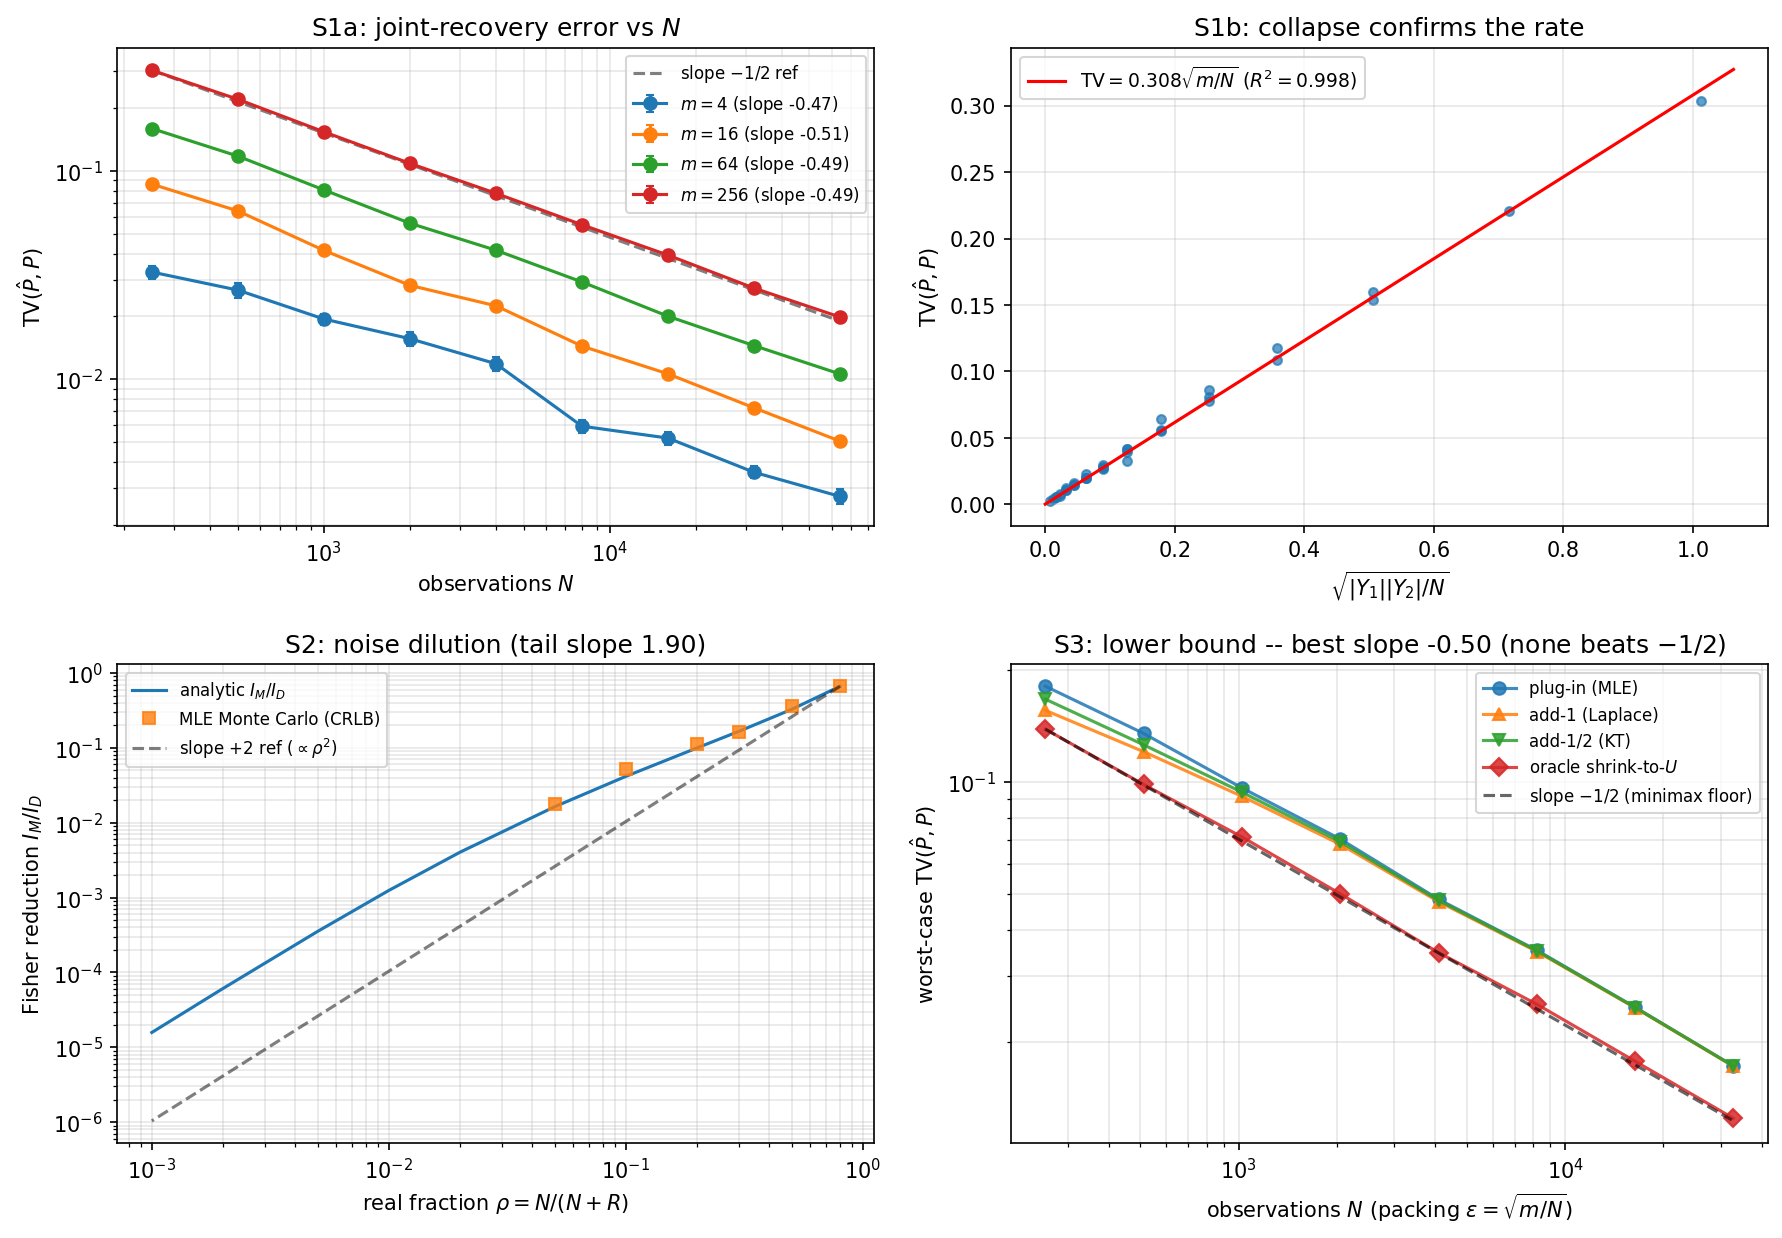
\includegraphics[width=\linewidth]{compositional_rate}
\caption{Monte Carlo validation ($40$ seeds/cell).
\textbf{Top left}: joint-recovery error $\TV(\hat P, P)$ versus $N$,
log-log, one line per support size $m = |Y_1||Y_2|$; fitted slopes
near $-1/2$.
\textbf{Top right}: the same data collapses onto
$\TV = 0.31\sqrt{m/N}$ ($R^2 = 0.997$), confirming the
$\Theta(\sqrt{|Y_1||Y_2|/N})$ rate of
Theorems~\ref{thm:comp-leakage}--\ref{thm:comp-leakage-lb}.
\textbf{Bottom left}: noise-injection Fisher reduction $I_M/I_D \propto
\rho^2$ (Theorem~\ref{thm:noise-dilution}); the analytic factor and the
efficient MLE (Cram\'er--Rao) agree, with the small-$\rho$ slope
approaching $+2$.
\textbf{Bottom right}: lower-bound sharpness
(Theorem~\ref{thm:comp-leakage-lb}); four estimators on the
minimax-calibrated Assouad packing, all decaying at slope $-1/2$, the
oracle cheater included: none beats the rate.}
\label{fig:montecarlo}
\end{figure}

\subsection{Realized Attack on the Construction}
\label{subsec:realized}

The Monte Carlo of~\S\ref{subsec:montecarlo} validates the recovery
rate in the abstract sampling model: i.i.d.\ draws from a known joint.
We close the loop by mounting the attack on cipher maps the
\texttt{trapdoor-maps} library actually builds.  Two maps $\fhat_1,
\fhat_2$ for latent $f_1, f_2 : X \to \{0,\ldots,7\}$ over a shared
domain $|X| = 4096$ are constructed with the PHF backend; the trusted
machine encodes inputs $x_i \mapsto c_i$, the untrusted machine
evaluates both maps on each shared cipher value, and the joint over
$Y_1 \times Y_2$ ($m = 64$) is recovered by plug-in
(Fig.~\ref{fig:realized}; $12$ seeds).

\paragraph{The construction reproduces the rate.}
At exact correctness ($\eta = 0$), the realized recovery error obeys
$\TV(\hat P, P) = c\sqrt{m/N}$ with slope $-0.50$ in $N$ and constant
$c = 0.32$, matching the abstract value $0.31$ of
\S\ref{subsec:montecarlo} to within seed noise
(Fig.~\ref{fig:realized}, right).  The hashing, acceptance predicates,
and finite cipher width of the real construction do not change the
$\Theta(\sqrt{|Y_1||Y_2|/N})$ leakage rate: the abstract theorem
describes the deployed system.

\paragraph{Correctness sets a recovery floor.}
The correctness parameter $\eta$ (the fraction of elements that decode
incorrectly) bounds the attack from below: an $\eta$-fraction of
recovered pairs is corrupted, so $\TV(\hat P, P)$ does not vanish but
floors near $\eta$ (Fig.~\ref{fig:realized}, left: the $\eta = 0.05$
curve flattens at $\approx 0.050$ and $\eta = 0.02$ at $\approx 0.027$,
while the exact curve keeps falling past $0.020$).  This is the
defender's side of the deniability afforded by $\eta > 0$
(\S\ref{sec:prelim}): the same residual error that gives a real query
plausible deniability also caps how well an adversary can reconstruct
the compositional joint.

\begin{figure}[ht]
\centering
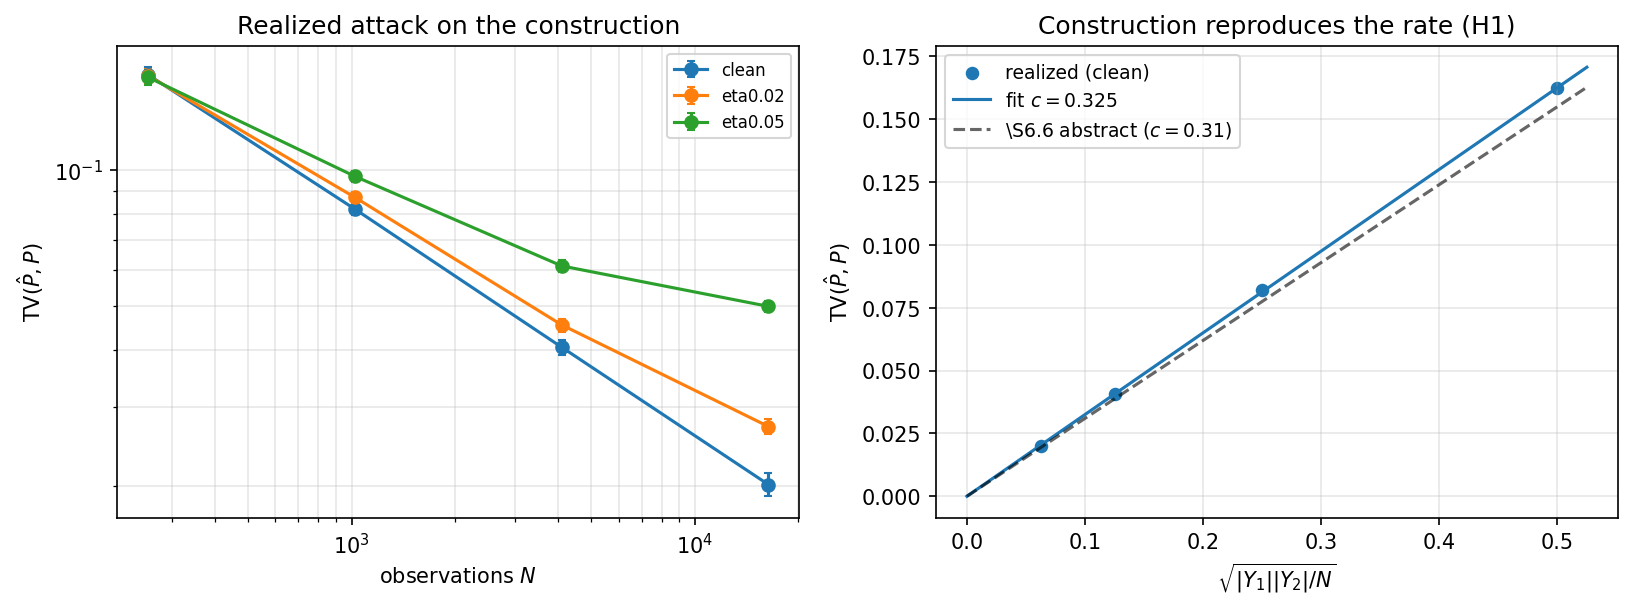
\includegraphics[width=\linewidth]{realized_attack}
\caption{Compositional attack on cipher maps built by the
\texttt{trapdoor-maps} library ($12$ seeds, $|X| = 4096$, $m = 64$).
\textbf{Left}: recovery error versus $N$ for three correctness levels;
the exact ($\eta = 0$) curve falls at slope $-1/2$, while $\eta > 0$
floors near $\eta$.
\textbf{Right}: the exact-construction error collapses onto
$\TV = 0.32\sqrt{m/N}$, matching the abstract-model constant $0.31$ of
\S\ref{subsec:montecarlo} (dashed): the real construction leaks the
joint at the predicted rate.}
\label{fig:realized}
\end{figure}

\subsection{Case Study: Confidentiality Improvement}

We demonstrate two of the levers of~\S\ref{sec:levers} (noise
injection and multiplicity) on a system with vocabulary
$m = 10{,}000$ and Zipf-distributed queries.  Table~\ref{tab:case-study}
gives the resulting entropy ratios under combinations of the two
levers.

\begin{table}[ht]
\centering
\caption{Confidentiality improvement via two of the levers of
\S\ref{sec:levers} (noise injection and multiplicity).  Values are
analytical, computed from the Zipf
entropy, the mixture-entropy formula in Theorem~\ref{thm:noise-dilution},
and the homophonic construction in Example~\ref{ex:homophonic}.}
\label{tab:case-study}
\resizebox{\columnwidth}{!}{%
\begin{tabular}{@{}lrrr@{}}
\toprule
Configuration & $e$ & Space overhead & Bandwidth overhead \\
\midrule
Baseline (simple substitution) & 0.72 & $1.00\times$ & $1.00\times$ \\
+ Homophonic ($b = 100$, $c \approx 979$) & 0.87 & $1.05\times$ & $1.00\times$ \\
+ Noise injection ($R/N = 0.5$) & 0.84 & $1.00\times$ & $1.50\times$ \\
Combined & 0.94 & $1.05\times$ & $1.50\times$ \\
Theoretical maximum & 1.00 & $\to \infty$ & $\to \infty$ \\
\bottomrule
\end{tabular}%
}
\end{table}

The combined strategy improves $e$ from 0.72 to 0.94: a 5\% space
overhead and 50\% bandwidth overhead yields a 22 percentage point
confidentiality improvement.  (The noise rows use the exact mixture
entropy $H(\rho D + (1-\rho)U_{\mathrm{im}})$ of
Theorem~\ref{thm:noise-dilution}, not the source-plus-indicator sum,
which would over-credit by the unobserved real/filler label.)  The small
space cost reflects the
classical homophonic prescription $K(x) \propto D(x)$: concentrating
multiplicity on the heavy part of $D$ is far cheaper than the inverse
allocation $K(x) \propto 1/D(x)$, which would spend
$\sum_x K(x) \approx c \cdot m \cdot H_m$ slots flattening the tail
(and, by the sampling identity $Q(c) = D(x)/K(x)$, would in fact
\emph{sharpen} the cipher-value distribution rather than flatten it).


%% ====================================================================
\section{Discussion and Open Questions}
\label{sec:discussion}
%% ====================================================================

\paragraph{The entropy ratio as a design tool.}
The entropy ratio $e$ gives system designers a single number to
optimize.  Given a resource budget (space $S$, bandwidth $B$), the
designer solves: maximize $e$ subject to $\text{space} \leq S$ and
$\text{bandwidth} \leq B$.  The framework's three levers (noise
injection, multiplicity, granularity), whose costs we analyze here,
provide the degrees of freedom.  Noise costs bandwidth but not space;
multiplicity costs space but not bandwidth; granularity trades
confidentiality for functionality.

\paragraph{Shannon entropy vs.\ min-entropy.}
We adopt Shannon entropy because the adversary in our setting observes
many cipher values and estimates a distribution over them: a
distribution-estimation problem rather than a single-query guessing
problem.  Smith~\cite{smith2009foundations} argues that min-entropy
leakage $L_\infty = -\log_2 \max_x P(X = x \mid \mathrm{view})$ is the
correct measure when one high-probability outcome dominates and the
adversary has a single guess.  In a cipher map system, that scenario
arises when a single query is overwhelmingly likely; the entropy ratio
can be high even when one cipher value is identifiable, so a Shannon
bound does not preclude min-entropy leakage of that one value.  The
min-entropy analogue of Theorem~\ref{thm:entropy-decomposition} would
replace $\delta$-closeness in TV with $\ell_\infty$-closeness
$\delta_\infty = \max_c |Q(c) - U(c)|$ and yield a min-entropy bound
$H_\infty(Q) \geq n - \log_2(1 + 2^n \delta_\infty)$.  Constructing
cipher maps with bounded $\delta_\infty$ rather than $\delta$ is
strictly harder (it constrains the worst-case cell, not the average),
and the multiplicity construction $K(x) \propto D(x)$ does not by
itself guarantee small $\delta_\infty$.  We leave a full min-entropy
treatment to future work; Shannon suffices for the average-case
adversary that motivates this paper.

\paragraph{Relationship to the orbit closure.}
The entropy ratio measures \emph{passive} confidentiality: what the
adversary learns by observing the cipher value stream.  The orbit closure
from~\cite{towell2026algebraic} measures \emph{active} confidentiality:
what the adversary learns by applying the cipher maps it holds.  A
complete confidentiality analysis requires both: high $e$ (passive) and
small orbit (active).  Connecting these two measures---showing that high
$e$ implies small effective orbit under certain conditions---is an open
problem.

\paragraph{Practical depth in cipher programs.}
A useful cipher program is typically structured in two layers: a
trusted-side orchestrator (e.g., a Python control loop) that decides
which cipher map to invoke and in what order, and a set of cipher-map
primitives (membership, comparison, lookup, conjunction) that the
untrusted machine evaluates blindly on cipher values.  How deep can
the call chain through the untrusted machine go?  The framework does
not impose a structural ceiling, but two confidentiality budgets
constrain practical depth.  First, FPR compounding
(Appendix~\ref{subsec:fpr-compounding}) imposes a correctness ceiling:
after roughly $k = 3$ AND levels at $p_T = 0.05$, the empirical
false-positive rate hits a construction-level noise floor of about
$4 \times 10^{-3}$ (Table~\ref{tab:fpr}); deeper AND chains cannot
drive precision below this floor.  Second, each chain level exposes
an additional intermediate cipher value to the untrusted machine,
which combines with Theorem~\ref{thm:comp-leakage} (compositional
leakage from shared variables) and the orbit-closure
bound~\cite[Thm.~5.3]{towell2026algebraic} to erode confidentiality
super-linearly with depth.  Empirically (\S\ref{subsec:granularity})
the leaf encoding of a 7-function pipeline exposes seven
intermediate cipher values per query, against the root encoding's
one; the Theorem~\ref{thm:comp-leakage-lb} minimax rate then gives
the adversary a sharper joint estimator at the leaf level.  In
practice, useful cipher programs span depth 2--5: end-to-end
encrypted Boolean search at depth 2--3 (cipher membership plus
cipher AND/OR), cipher decision trees at depth equal to the tree
depth, and analytics pipelines at depth 3--5 (filter, aggregate,
threshold).  Beyond depth 5 the granularity-vs-leakage trade-off
typically argues for re-rooting the chain: collapse the deep
sub-pipeline into a single cipher map for the joint computation, at
the space cost of $O(|Y|^k)$ from Proposition~\ref{prop:granularity}.
A third budget applies when a program reuses the \emph{same}
primitive across many cipher values (e.g.\ a comparison applied at
every node of a wide query): the multi-instance coincidence
oracle~\cite[Thm.~8.2]{towell2026cipher} lets the untrusted machine
accumulate evidence about a shared latent value at accuracy growing
with the number of instances, a channel orthogonal to chain depth and
likewise uncontrolled by $\delta$.  Concentrated acceptance partitions
and randomized encoding ($K(x) > 1$) are the defenses there.

\paragraph{Adaptive $K(x)$.}
The multiplicity $K(x)$ is set at construction time based on an assumed
distribution $D$.  If $D$ changes over time (e.g., query distribution
shift), the system loses uniformity.  Adaptive $K(x)$ that adjusts to
observed frequencies without reconstruction would improve robustness.
This requires an online construction strategy where representations can
be added incrementally.

\paragraph{Tight bounds for composition.}
The general composition theorem gives
$\eta_{g \circ f} \leq 1 - (1 - \eta_f)(1 - \eta_g)$ under
independence.  For specific circuits (e.g., 3-SAT evaluation over cipher
Booleans), the actual error rate depends on the input distribution and
the circuit structure.  Case-by-case interval arithmetic gives tighter
bounds but does not scale.  Automated analysis tools that propagate
entropy through circuit DAGs would be useful.

\paragraph{Beyond Boolean search.}
This paper focuses on encrypted Boolean search as the primary
application.  The cipher map framework supports arbitrary functions
$f : X \to Y$, and the confidentiality theory extends naturally.  Ranked
retrieval (scoring functions), phrase search (bigram models), and
approximate string matching all admit cipher map implementations with
different confidentiality profiles.

\paragraph{Limitations.}
\begin{enumerate}
\item The entropy ratio is an average measure; it does not bound the
  leakage of any \emph{specific} query.  A single high-frequency query
  may be identifiable even when $e$ is close to 1.

\item Compression-based estimation is positively biased (overestimates
  confidentiality).  The bias decreases with sequence length but can be
  significant for short sequences.

\item The analysis assumes the random oracle model for cryptographic
  hashing.  In practice, hash functions have biases that may reduce
  confidentiality below the theoretical predictions.

\item Marginal uniformity ($\delta \approx 0$) is necessary but not
  sufficient.  Joint distributions, temporal patterns, and side channels
  (timing, bandwidth) can leak information that the entropy ratio does
  not capture.
\end{enumerate}


%% ====================================================================
\section{Conclusion}
\label{sec:conclusion}
%% ====================================================================

We have developed a quantitative confidentiality theory for cipher map
systems, grounded in the cipher map framework
of~\cite{towell2026cipher}.  The headline result is the compositional
leakage pair (Theorems~\ref{thm:comp-leakage}
and~\ref{thm:comp-leakage-lb}): even when each cipher map's marginal
cipher distribution is $\delta$-uniform, observing multiple
evaluations on a shared cipher value lets the untrusted machine
recover the latent joint at the information-theoretically optimal
rate $\Theta(|Y_1|\cdot|Y_2|/\xi^2)$, with matching upper bound from
plug-in estimation and matching lower bound via Assouad's lemma.
No per-cipher-map parameter changes the rate, so marginal
uniformity is necessary but not sufficient; the cipher map composition
discipline that buys functionality also creates an information
channel through shared values, and only system-level interventions
(observation limits, joint encoding, or noise injection) reduce the
adversary's effective advantage at this scale.

To make the marginal target itself operational, we connect $\delta$ to
the entropy ratio $e = H/H^*$ (a normalized form of Shannon leakage
borrowed from the QIF literature) via the Fannes--Audenaert continuity
inequality, reducing marginal-leakage engineering to minimizing
$\delta$.  The framework's three $\delta$-reduction mechanisms come
with explicit costs that we characterize: noise injection (bandwidth),
multiple representations with $K(x) \propto D(x)$ (space), and encoding
granularity (the $O(|Y|^k)$ correlation-hiding trade-off).  The
constructions are the framework's; the cost analysis, and the
Fisher-information dilution of noise injection, are ours.  The three
are expressible in terms of the cipher map parameters
$(\eta, \varepsilon, \mu, \delta)$ and the entanglement parameter $p$.

The key insight is that the cipher map's four properties already
determine the confidentiality profile.  Totality enables noise injection
(filler queries are indistinguishable from real queries).  Representation
uniformity enables frequency hiding (multiple representations flatten the
distribution).  Composability enables chained evaluation but introduces
correlation leakage---the very channel exploited by Theorem~\ref{thm:comp-leakage}.
Correctness provides plausible deniability
($\eta > 0$ means the adversary cannot be certain of any decoded output).

Experimental validation on the 20 Newsgroups corpus bears out the theory
and its limits: OR-chain FPR matches $1 - (1 - p_T)^k$, while AND chains
fall to a construction-level noise floor ($\approx 4 \times 10^{-3}$)
rather than continuing as $p_T^k$, which we read as a defender's
confidentiality budget; the encoding granularity spectrum trades one
exposed cipher value per query at root granularity (37.0 bits/element)
against seven at leaf granularity (7.5 bits/element per map); and the
combined homophonic/noise strategy improves confidentiality from 72\% to
94\% with approximately $1.05\times$ space and $1.5\times$ bandwidth
overhead.

The theory connects two previously separate lines of work: the cipher map
formalism (properties and composition) and the entropy-based
confidentiality analysis (ratios and maximum entropy).  Together, they
give a principled basis for designing, measuring, and improving
confidentiality in systems that compute on data hidden behind a trapdoor,
at both the marginal and the compositional scale.



\appendices
\label{app:start}

\section{Practical Measurement}
\label{sec:measurement}
%% ====================================================================

\subsection{Compression-Based Entropy Estimation}

The entropy of a sequence can be estimated without an explicit
probabilistic model by compressing it.  This follows from Shannon's
source coding theorem~\cite{shannon1948mathematical}: the expected length
of the output of an optimal lossless compressor equals the entropy of the
source.

\begin{proposition}[Compression estimator]
\label{prop:compression}
Let $\mathbf{c} = (c_1, \ldots, c_N)$ be a sequence of cipher values
observed by the untrusted machine, encoded as a bit string via some
fixed encoding $\mathrm{Encode}$.  Let $\mathrm{Compress}$ be a lossless
compressor.  Then:
\begin{equation}
\hat{H} = \frac{|\mathrm{Compress}(\mathrm{Encode}(\mathbf{c}))|}{N}
\end{equation}
is a positively biased estimator of the per-element entropy
$H(C_1, \ldots, C_N) / N$.  That is, $\hat{H} \geq H/N$ in expectation,
with equality when $\mathrm{Compress}$ is optimal.
\end{proposition}

\begin{proof}
A uniquely decodable code on $\mathbf{c}$ of length
$L(\mathbf{c}) = |\mathrm{Compress}(\mathrm{Encode}(\mathbf{c}))|$
satisfies the Kraft inequality and induces a probability measure
$Q(\mathbf{c}) \leq 2^{-L(\mathbf{c})}$.  The expected codelength
satisfies $\mathbb{E}_P[L(\mathbf{c})] \geq H(C_1, \ldots, C_N)$ by
the source-coding theorem~\cite{shannon1948mathematical}, with the gap
equal to the divergence $D_{\mathrm{KL}}(P \| Q) \geq 0$ (cross-entropy
inequality, see~\cite[Thm.~5.4.3]{cover2006elements}).  Equality holds
when the compressor matches the source distribution; for universal
compressors (e.g., LZ77, LZ78), the per-symbol gap vanishes
asymptotically as $N \to \infty$~\cite{shannon1948mathematical}.
Dividing by $N$ gives $\hat{H} \geq H/N$ in expectation.  The
encoding overhead is bounded by a constant factor (any uniquely
decodable encoding has a bounded prefix), so it contributes
$O(1/N)$ to the per-symbol bias and vanishes in the same limit.
\end{proof}

The compression estimator has three practical advantages:
\begin{enumerate}
\item It requires no model of the query distribution.
\item It captures all forms of structure (frequency, correlation,
  temporal patterns) that a lossless compressor can detect.
\item It is cheap to compute: a single pass through the data with
  \texttt{gzip} or \texttt{zstd}.
\end{enumerate}

\paragraph{Entropy ratio estimator.}
Given the compression-based estimate $\hat{H}$ and a computable
$H^*$ (from the system parameters), the entropy ratio is estimated as:
\begin{equation}
\hat{e} = \frac{\hat{H}}{H^*}.
\end{equation}
Since $\hat{H}$ is positively biased, $\hat{e}$ is also positively
biased (overestimates confidentiality).  This is the conservative
direction: the system is at least as confidential as the estimate suggests.

\subsection{Monte Carlo Estimation}

When the query distribution is available (e.g., from historical logs),
entropy can be estimated by sampling.  Generate $M$ independent query
sequences of length $N$, compute the cipher value distribution, and
estimate $H$ directly:
\begin{equation}
\hat{H}_{\mathrm{MC}} = -\sum_v \hat{p}(v) \log_2 \hat{p}(v),
\end{equation}
where $\hat{p}(v)$ is the empirical frequency of cipher value $v$ across
the $M$ samples.  This estimator is negatively biased for finite $M$
(the Miller--Madow correction adds $(\hat{m} - 1) / (2M \ln 2)$ where
$\hat{m}$ is the number of distinct observed values), but converges to
the true entropy as $M \to \infty$.

\subsection{The Leakage Analyzer}

We define the \emph{leakage analyzer} as the procedure that combines
compression-based and Monte Carlo estimation:
\begin{enumerate}
\item Observe or simulate a sequence of cipher values.
\item Compute $\hat{H}$ via compression and $\hat{H}_{\mathrm{MC}}$ via
  sampling (if the distribution is available).
\item Compute $H^*$ from the system parameters using the maximum entropy
  formulas.
\item Report $\hat{e} = \hat{H} / H^*$ and the entropy gap
  $H^* - \hat{H}$ in bits.
\end{enumerate}
The entropy gap quantifies how many bits of information per query the
adversary potentially gains from the non-uniformity of the system.

\subsection{Finite-Sample Resolution of \texorpdfstring{$\delta$}{delta}}
\label{subsec:finite-sample}

The estimators above measure entropy.  The representation-uniformity
parameter $\delta = \TV(Q, U)$ can also be measured directly from
observed cipher values, but only at a query cost that scales with the
allocated budget.

Let $|\im| = \sum_x K(x)$ denote the image size of $\enc$ under a given
homophonic allocation, and let $\hat{Q}_N$ be the empirical
distribution over the image after observing $N$ cipher values.  By the
multinomial $\ell_1$/TV concentration
bound~\cite{devroye1996nonparametric},
$\TV(\hat{Q}_N, Q) = O(\sqrt{|\im|/N})$, so the
empirical estimator $\hat{\delta}_N = \TV(\hat{Q}_N, U)$ has
finite-sample bias of the same order:
\begin{equation}
\hat{\delta}_N - \delta \;=\; O\!\left(\sqrt{|\im|/N}\right).
\label{eq:finite-sample-bias}
\end{equation}

To resolve $\delta$ at a target level $\delta_0$ thus requires
\begin{equation}
N \;=\; \Omega\!\left(|\im| / \delta_0^2\right)
\label{eq:n-required}
\end{equation}
observed cipher values.  This is a practical lower bound on the
evaluation cost of any cipher map system claiming a particular
$\delta$: increasing the budget $\sum K$ improves the analytical
floor (Theorem~\ref{thm:multiplicity}) but proportionally increases
the query stream length needed to verify the improvement.

We confirm this empirically by sweeping a $(\sum K, N)$ grid on a
synthetic Zipf distribution and measuring
$\hat{\delta}_N - \delta_{\mathrm{predicted}}$
across cells (Fig.~\ref{fig:finite-sample-gap}).  The gap fits a
linear law $\hat{\delta}_N - \delta \approx 0.4\sqrt{|\im|/N}$ across
budgets in $[32, 2048]$ and stream lengths in $[500, 50{,}000]$.

\begin{figure}[ht]
\centering
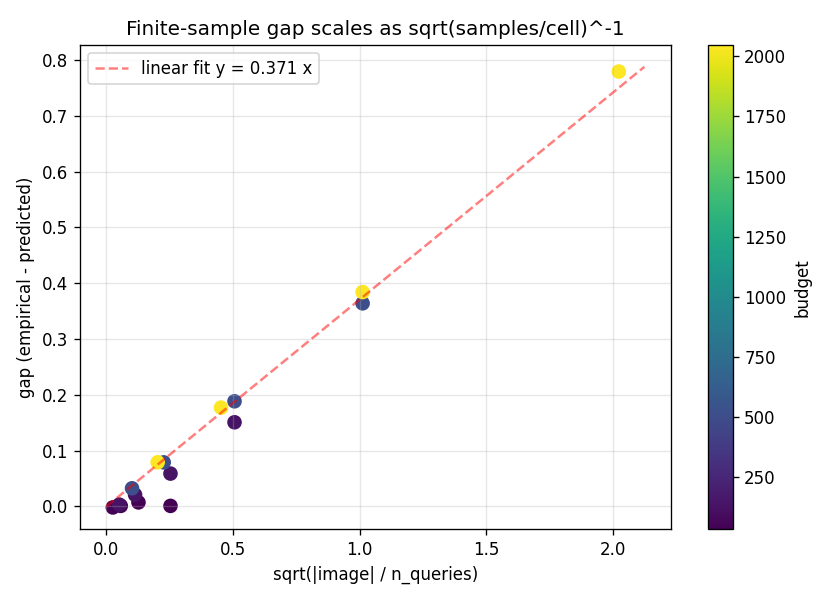
\includegraphics[width=0.85\linewidth]{finite_sample_gap}
\caption{Finite-sample bias of $\hat{\delta}_N$ as a function of
$\sqrt{|\im|/N}$.  Each point is the mean over three replicates of a
proportional homophonic allocation on Zipf$(32, \alpha=1.5)$; colour
encodes total budget.  The dashed line is the origin-anchored linear
fit, slope $\approx 0.4$.}
\label{fig:finite-sample-gap}
\end{figure}

\paragraph{Practical implication.}
A defender increasing $\sum K$ to drive analytical $\delta$ from
$10^{-2}$ to $10^{-3}$ must also increase the validation query
budget from roughly $10^4 |\im|$ to $10^6 |\im|$, a hundredfold
growth.  Below this threshold the empirical estimate $\hat{\delta}_N$
is dominated by sampling noise and will overstate leakage.

\subsection{Empirical Anchor for the Compression Estimator}
\label{subsec:compression-validation}

Proposition~\ref{prop:compression} states that gzip-style
compression yields a positively-biased estimator $\hat H$ of the
per-symbol entropy.  We anchor this prediction empirically across
three synthetic streams (i.i.d.\ uniform sanity check, first-order
Markov auto-correlation, and the noise mixture of
Theorem~\ref{thm:noise-dilution}) plus one real-corpus stream
(20 Newsgroups token sequence).  Synthetic streams use 16-bit
cipher values ($n = 16$, byte-aligned for gzip) and are averaged
over $5$ random seeds.

\begin{figure}[ht]
\centering
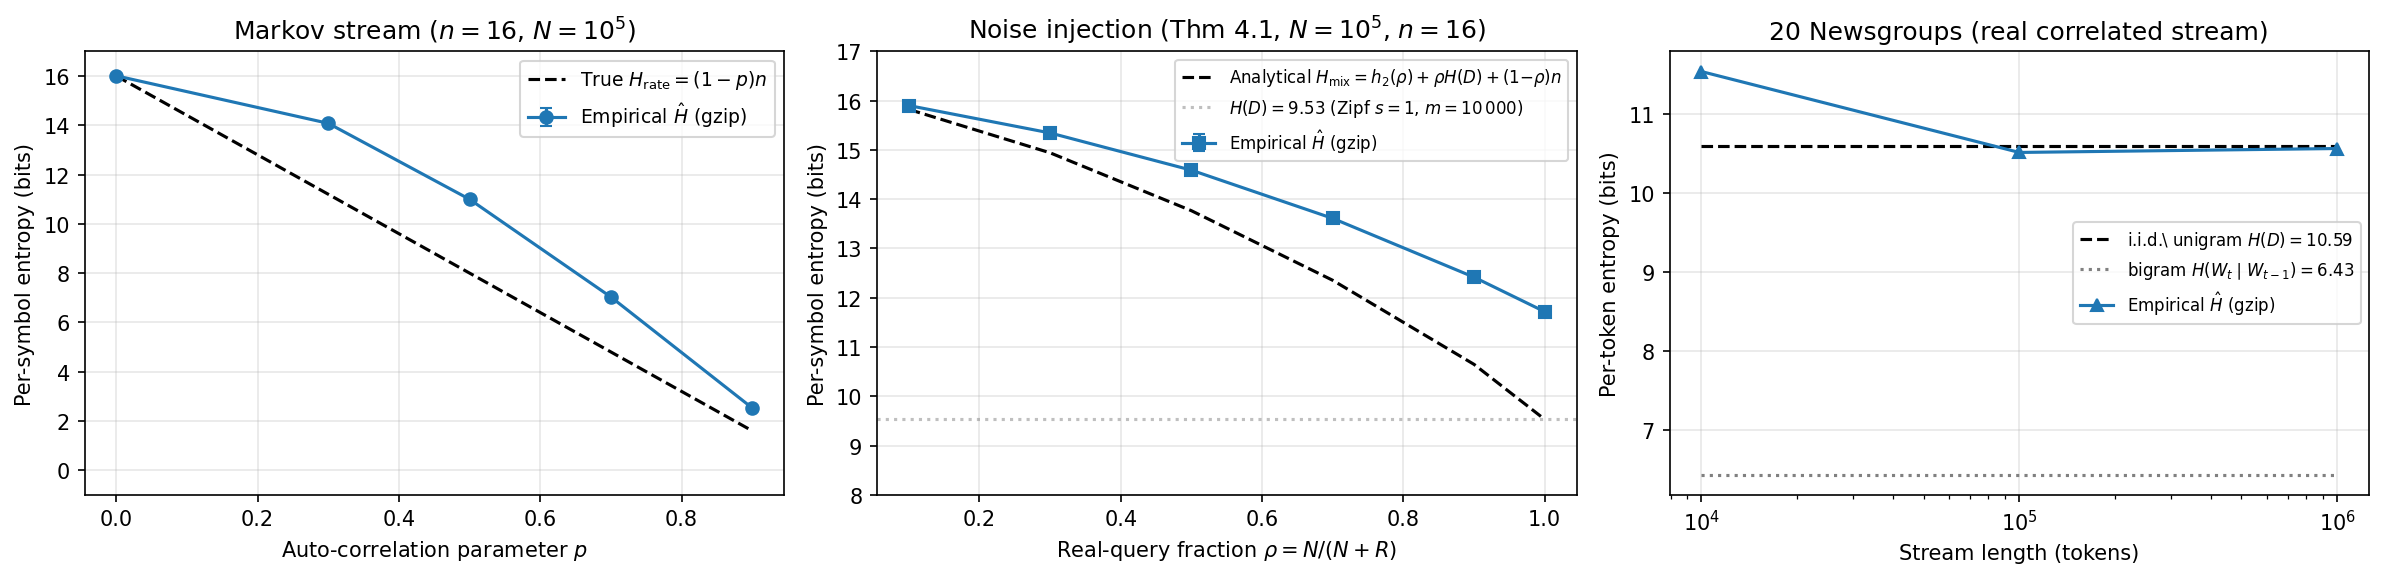
\includegraphics[width=\linewidth]{compression_validation}
\caption{Compression-based entropy estimation against analytically
known entropy rates and a real-corpus reference.
\textbf{Left}: first-order Markov stream ($n = 16$, $N = 10^5$,
5 seeds, error bars $\pm 1\sigma$) with auto-correlation parameter
$p$, entropy rate $H_{\mathrm{rate}} = (1-p)n$.
\textbf{Centre}: real Zipf queries ($s=1$, $m = 10\,000$) mixed
with uniform filler at fraction $\rho$, predicted entropy
$H_{\mathrm{mix}} = h_2(\rho) + \rho H(D) + (1-\rho)n$ from
Theorem~\ref{thm:noise-dilution}.
\textbf{Right}: 20 Newsgroups token stream (uint16-capped
encoding) versus the i.i.d.\ unigram entropy $H(D)$ and the
empirical bigram conditional entropy $H(W_t \mid W_{t-1})$ as a
model-based reference.  Stream length on log scale.}
\label{fig:compression-validation}
\end{figure}

Figure~\ref{fig:compression-validation} shows the results.  The
sanity check is omitted from the figure for clarity but is reported
here: on i.i.d.\ uniform streams of length $N = 10^5$, $\hat H = 16.007 \pm 0.000$ bits, a bias of $7 \times 10^{-3}$ bits per
symbol attributable to gzip's header.

\paragraph{Markov auto-correlation (left panel).}
The estimator tracks the predicted $H_{\mathrm{rate}}$ across the
full range $p \in [0, 0.9]$, dropping from $\approx 16$ bits at
$p = 0$ (i.i.d.\ uniform) to $\approx 2.5$ bits at $p = 0.9$
(highly redundant).  Bias is consistently positive (1--3 bits) and
peaks near $p \approx 0.5$, reflecting gzip's byte-level dictionary
on a 16-bit-symbol source: when half the stream is repeated, gzip's
LZ77 backreferences capture the structure but Huffman entropy on
the literal pairs adds overhead.  The estimator's slope is correct
even where its absolute level is biased: a defender comparing two
configurations would see the relative ordering preserved.

\paragraph{Noise mixture (centre panel).}
The mixture panel tests Theorem~\ref{thm:noise-dilution}'s
formula on its own terms: both real (Zipf) and filler (uniform)
draws are i.i.d., matching the i.i.d.\ assumption Theorem~\ref{thm:noise-dilution}
makes.  The estimator tracks $H_{\mathrm{mix}}$ from $\rho = 0.1$
($\hat H = 15.90$, predicted $15.82$) to $\rho = 1.0$ pure Zipf
($\hat H = 11.72$, predicted $9.53$).  Bias grows monotonically
with $\rho$ because i.i.d.\ Zipf queries have no temporal structure
for LZ77 to exploit; in the pure-Zipf regime gzip degenerates into
a byte-level Huffman coder, and the byte-pair entropy of 16-bit
Zipf samples is higher than the 14-bit symbol entropy of the
underlying distribution.  Adding filler dilutes this confound.

\paragraph{Real corpus (right panel).}
Real query streams are not i.i.d.: natural-language queries have
sessional repetition, topical bursts, and grammatical structure
that an i.i.d.\ analysis cannot capture.  The 20 Newsgroups
training split provides such a stream: $2.31\,\text{M}$ tokens of
natural English, encoded as uint16 token IDs (vocab capped at
65{,}535).  Two model-based references bound the entropy rate from
above and below: the i.i.d.\ unigram entropy
$H(D) = 10.59$ bits/token (computed from the empirical word
frequencies), and the first-order Markov conditional entropy
$H(W_t \mid W_{t-1}) = 6.43$ bits/token (computed from empirical
bigram counts).

The compression estimator lands at $\hat H \approx 10.56$ bits per
token at $N = 10^6$, just below the i.i.d.\ bound of $10.59$.
gzip therefore detects \emph{some} of the natural-language
correlation that an i.i.d.\ unigram analysis would miss, but the
margin is small (roughly $0.03$ bits, near the noise floor of
single-corpus measurement).  The bigram model-based estimate of
$6.43$ bits/token sits four bits below $\hat H$, indicating that
gzip's LZ77 window and Huffman literal coding miss most of the
deeper grammatical and topical structure.  Encoding choice matters:
the same stream encoded as uint32 yields $\hat H \approx 12.16$
bits/token (worse than the i.i.d.\ bound, because two of the four
bytes are mostly zero and inflate the per-token cost).  A tight
encoding is necessary for the estimator to be informative at all.

\paragraph{Operational reading.}
Three lessons emerge.  First, the bias direction matches
Proposition~\ref{prop:compression} on every stream: $\hat H$ is an
upper bound on the entropy rate, never below it.  Second,
gzip's value as an absolute estimator is sharply limited by both
the input encoding and the compressor's effective context window:
on the 20NG token stream, gzip captures only the marginal symbol
distribution (matching the i.i.d.\ unigram bound to within
$0.03$ bits) and misses the bigram structure that brings the true
entropy rate down by four bits.  For absolute Shannon-entropy
measurements on cipher-value streams a model-based estimator
(context-tree weighting~\cite{cover2006elements}, or higher-order
Markov models) is preferable.  Third, gzip remains useful for
\emph{relative} measurements: the Markov panel shows $\hat H$
tracks $H_{\mathrm{rate}}$'s slope across the full
$p \in [0, 0.9]$ range, and the noise-mixture panel shows $\hat H$
tracks $H_{\mathrm{mix}}$'s slope across $\rho$.  Operators
tracking confidentiality changes over time should fix the
estimator and compare $\hat H$ trajectories rather than read
absolute values.

\paragraph{Scope: stream archetypes, not specific cipher programs.}
The four streams above test $\hat H$ on archetypes of structure
(i.i.d.\ uniform, first-order Markov, i.i.d.\ mixture, real
correlated text), not on the cipher-value output of any specific
multi-primitive cipher program.  For a single-cipher-map system
the adversary's stream is a sequence of cipher values from one
cipher map and the validation here applies directly.  For a
compositional cipher program (cipher Boolean queries
of~\S\ref{sec:experiments}, depth-$k$ Boolean chains, or richer
pipelines) the adversary's stream is a concatenation of cipher
values from multiple cipher maps, with structure shaped by the
program's call pattern and by the compositional leakage of
Theorem~\ref{thm:comp-leakage}.  Validating $\hat H$ on
program-specific streams would require a separate
program-by-program study; this paper establishes the measurement
tool against generic archetypes and leaves the program-shape
mapping to deployment-time analysis.



%% ====================================================================

\section{Error Compounding in Boolean Chains}
\label{app:boolean}
\label{subsec:fpr-compounding}

For Boolean-valued cipher maps (e.g., set indicator functions
$\hat{1}_A : \cipher{X} \to \cipher{\mathrm{Bool}}$, or any
$\fhat$ with $Y = \{\mathrm{True}, \mathrm{False}\}$), the
composition behavior depends on the gate type.  Let $p_T$ denote the
\emph{false positive rate} (FPR):
\[
p_T = \Pr[\dec(\fhat(\enc(x,k))) = \mathrm{True} \mid f(x) = \mathrm{False}],
\]
the probability that an element with $f(x) = \mathrm{False}$ is
decoded as True.
For in-domain elements with $\eta = 0$, FPR is zero by construction.
For out-of-domain elements (not in the construction domain), the hash
output is effectively random and lands in the True region with
probability $|T|/2^n$.

\begin{proposition}[FPR compounding]
\label{thm:fpr-compounding}
For $k$ independent Boolean-valued cipher maps composed via Boolean
operations:
\begin{align}
\text{AND of } k \text{ tests:} &\quad
  \mathrm{FPR}_{\mathrm{total}} = p_T^k, \\
\text{OR of } k \text{ tests:} &\quad
  \mathrm{FPR}_{\mathrm{total}} = 1 - (1 - p_T)^k.
\end{align}
These follow from independence of the gate inputs (elementary).  The
gate-type framing is from the cipher maps
paper~\cite[Sec.~7.4]{towell2026cipher}; the explicit closed forms and
their empirical validation, including the construction-level noise
floor discussed below, are reported in the algebraic cipher types
paper~\cite[Table~3]{towell2026algebraic}.
\end{proposition}

AND drives false positive rate down exponentially: each additional
conjunct is an independent filter.  OR drives it up: each additional
disjunct adds false positive mass.  NOT is approximate due to
complement non-preservation via the pigeonhole
principle~\cite{towell2026cipher}.

\paragraph{Effect on confidentiality.}
AND chains improve precision (fewer false positives) but maintain the
same recall (elements with $f(x) = \mathrm{True}$ pass all tests).
From a confidentiality perspective, AND chains reduce the effective noise
level: with $p_T = 0.05$ and $k = 3$, the FPR drops to
$0.05^3 \approx 0.000125$, meaning almost all decoded True outputs
correspond to elements where $f(x) = \mathrm{True}$.
The adversary can infer with higher confidence that a True result is
correct (lower entropy ratio $e$), a direct trade-off between precision
and confidentiality.

OR chains have the opposite effect: FPR increases, adding noise to the
output stream.
The adversary's uncertainty grows (higher $e$), but the system returns
more false positives, reducing its usefulness.

\paragraph{Convergence under deep composition.}
Long AND chains converge toward False (or noise).
With $p_T = 0.05$ and $p_F = 0.90$, each AND step multiplies the
probability of a True result by $p_T$ for noise inputs.
After $k$ ANDs with independent random cipher values, the probability
of a True output is at most $p_T^k$, which vanishes rapidly.
The cipher Boolean output after a deep AND chain is almost certainly
False or noise, regardless of the initial value.
This limits the depth of useful AND composition: beyond a few
terms, the signal (legitimate True results) is indistinguishable from
the False/noise floor.

Dually, long OR chains converge toward True (or noise).
Each OR step with an independent input produces True with probability
at least $p_T$, and after $k$ steps the probability of \emph{not} seeing
True is at most $(1 - p_T)^k$.
Deep OR chains saturate at True, again drowning the signal.

In both cases, noise acts as an attractor: AND pulls toward False/noise,
OR pulls toward True/noise.
The noise region prevents the adversary from distinguishing
``legitimately False after AND'' from ``noise-induced False,'' providing
a floor of uncertainty even in deep compositions.

\paragraph{Active probing via Boolean operations.}
Exposing AND and OR to the untrusted machine creates an orthogonal
confidentiality risk: the adversary can actively probe cipher values to
learn their latent meaning.
Given a cipher value $c$ and cipher AND, the adversary computes
$\mathrm{AND}(c, c)$.
Since cipher maps are deterministic, this always returns the same result
for a given $c$.
If the adversary also has cipher values $c_1, c_2$ and computes
$\mathrm{AND}(c_1, c_2)$, $\mathrm{AND}(c_1, c_1)$, and
$\mathrm{AND}(c_2, c_2)$, it can check whether the results are
structurally consistent with both being True, both False, or one of each.
Over many such probes, the adversary partitions cipher values into
equivalence classes that correspond to latent Boolean values.

This is exactly the orbit closure
attack~\cite[Sec.~5]{towell2026algebraic}: each Boolean operation
enlarges the orbit of reachable cipher values from $c$, and the
confidentiality degrades as
$\mathrm{conf}_F(c) \geq 1 - |\orbitF_F(c)|/|X|$.
The more operations the untrusted machine can apply, the larger the
orbit, the lower the confidentiality.
This creates a fundamental tension: exposing AND/OR/NOT enables
untrusted-side Boolean search (a functionality gain) but simultaneously
provides the adversary with tools to probe the cipher space
(a confidentiality cost).

One mitigation: \emph{typed composition chains}~\cite[Sec.~5.5]{towell2026algebraic}.
Instead of a single shared cipher Boolean space where AND can be
self-composed indefinitely, define a tower of distinct cipher spaces
$\cipher{\mathrm{Bool}}_0, \cipher{\mathrm{Bool}}_1, \ldots$
where $\mathrm{AND}_i$ maps from level $i$ to level $i+1$.
Without $\mathrm{AND}_{k}$, the chain terminates at depth $k$.
The orbit is bounded by $1 + k$ and the type system enforces the
limit at construction time.

%% ====================================================================

\section{Encrypted Boolean Search Evaluation}
\label{app:boolsearch}

Cipher sets are built for each document using 8-bit cipher Booleans
($p_T = 0.05$, $p_F = 0.90$, $p_N = 0.05$).  Table~\ref{tab:boolean}
reports precision, recall, and false-positive count for Boolean
queries on 5,000 documents, averaged over 5 random seeds (mean
$\pm$ standard deviation).  Plaintext queries on the same documents
achieve perfect precision and recall as expected; the cipher
columns show the noise the cipher Boolean parameters
$(p_T, p_F, p_N)$ introduce.

\begin{table}[ht]
\centering
\caption{Boolean search on 20 Newsgroups (5,000 documents, $n=5$
seeds).  All recalls except OR-style queries are 1.0 because cipher
Booleans have $p_F = 0.90$ ($\eta = 0.10$ false-negative rate per
clause) but the True region admits all true positives at the
$p_T = 0.05$ noise-decode rate.  OR queries lose recall when noise
matches the OR pattern.}
\label{tab:boolean}
\resizebox{\columnwidth}{!}{%
\begin{tabular}{@{}lcccr@{}}
\toprule
Query & Cipher Prec. & Cipher Rec. & Plaintext Prec./Rec. & Mean FP \\
\midrule
Single term  & $0.408 \pm 0.014$ & $1.000 \pm 0.000$ & $1.00$ & $233 \pm 13$ \\
2-term AND   & $0.262 \pm 0.024$ & $1.000 \pm 0.000$ & $1.00$ & $43 \pm 5$ \\
3-term AND   & $0.291 \pm 0.043$ & $1.000 \pm 0.000$ & $1.00$ & $15 \pm 3$ \\
OR           & $0.365 \pm 0.010$ & $0.959 \pm 0.010$ & $1.00$ & $437 \pm 16$ \\
OR-AND-NOT   & $0.330 \pm 0.008$ & $0.909 \pm 0.010$ & $1.00$ & $402 \pm 15$ \\
\bottomrule
\end{tabular}%
}
\end{table}

AND chains drive the false-positive count down monotonically
($233 \to 43 \to 15$), as predicted by the FPR compounding theory of
\S\ref{subsec:fpr-compounding} and confirmed in
Table~\ref{tab:fpr}.  Precision recovers slightly at $k=3$ (from
$0.262$ to $0.291$) because the smaller false-positive count is
diluted by a smaller true-positive count when the conjunction
becomes selective.  OR-style queries trade precision for noise:
they preserve the false positives of each disjunct, but their
larger result sets increase entropy from the adversary's view.
From a confidentiality perspective, the high-FP queries
(single-term, OR) yield more entropy in the result-set channel,
while AND chains return more deterministic results.



\section{Encoding Granularity (Experiment)}
\label{app:granexp}

Table~\ref{tab:granularity} shows the cost spectrum for encoding
a 7-function decision pipeline (loan approval) at three granularity
levels, using a domain of 150 inputs (30 applicants $\times$ 5 loan
amounts).

\begin{table}[ht]
\centering
\caption{Encoding granularity spectrum for a 7-function decision
pipeline (mean $\pm$ std over $n$ seeds; intermediate level has
$n=2$ successful runs because of construction failures at this
domain size on three of five seeds).  Bits/elem measures the
\emph{per-cipher-map} slot table cost; total exposed bits per
latent input is roughly bits/elem $\times$ exposed.}
\label{tab:granularity}
\resizebox{\columnwidth}{!}{%
\begin{tabular}{@{}lrrrrr@{}}
\toprule
Granularity & Build (s) & Space (B) & Bits/elem & Errors & Exposed \\
\midrule
Root ($p = 7$, $n=5$) & $0.003 \pm 0.000$ & $694$ & $37.0$ & $0$ & $1$ \\
Intermediate ($p \approx 3$, $n=2$) & $1.667 \pm 1.161$ & $138$ & $7.4$ & $0$ & $3$ \\
Leaf ($p = 1$, $n=5$) & $1.142 \pm 1.449$ & $140$ & $7.5$ & $0$ & $7$ \\
\bottomrule
\end{tabular}%
}
\end{table}

Per-cipher-map cost is dominated by the joint domain size: the root
encoding builds one cipher map over the 150-input $\times$ 7-output
joint space, paying 37 bits/element for one large slot table.  The
leaf and intermediate encodings build smaller cipher maps (one per
function or per group), each over a smaller joint space, so their
per-map bits/element are an order of magnitude lower (about
$7.5$).  But total \emph{exposed} cipher-map bits is the sum across
exposed maps: leaf exposes $7 \times \text{slot table}$, root
exposes $1 \times$.  Counting exposed cipher values rather than
per-map bytes recovers the asymmetry of the granularity spectrum:
the root encoding leaks one cipher value per latent query while the
leaf encoding leaks seven, so the per-query cipher-value entropy
the adversary observes is seven times larger at the leaf level.
The intermediate level's higher build variance reflects the bin
search this configuration performs at construction time; production
deployments would memoize the bin layout to avoid the variance.



\section{Homophonic Encoding Evaluation}
\label{app:homexp}
\label{subsec:newsgroups-homophonic}

We apply the proportional homophonic prescription
(Theorem~\ref{thm:multiplicity}) to the empirical word-frequency
distribution of the 20 Newsgroups training split.  Tokenising the
2.31\,M word corpus and retaining the top 500 most frequent words
gives a vocabulary in which the head word \emph{the} carries 7.1\%
of probability mass, the top ten words 33\%, and the top hundred
74\%.  The effective vocabulary $1/\sum_x D(x)^2$ is 64, so the
distribution is highly skewed even after tail truncation.

We compare three allocators across budgets $\sum K \in
\{|X|, 2|X|, 5|X|, 20|X|, 100|X|\}$: the uniform baseline
($K(x) = b/|X|$), the proportional homophonic
($K(x) \propto D(x)$), and a sub-optimal square-root variant
($K(x) \propto \sqrt{D(x)}$).  For each cell we build a fresh
\texttt{PHFCipherMap}, stream $N = 30{,}000$ queries sampled from
$D$, and record predicted and empirical TV
(Fig.~\ref{fig:newsgroups-homophonic}).

\begin{figure}[ht]
\centering
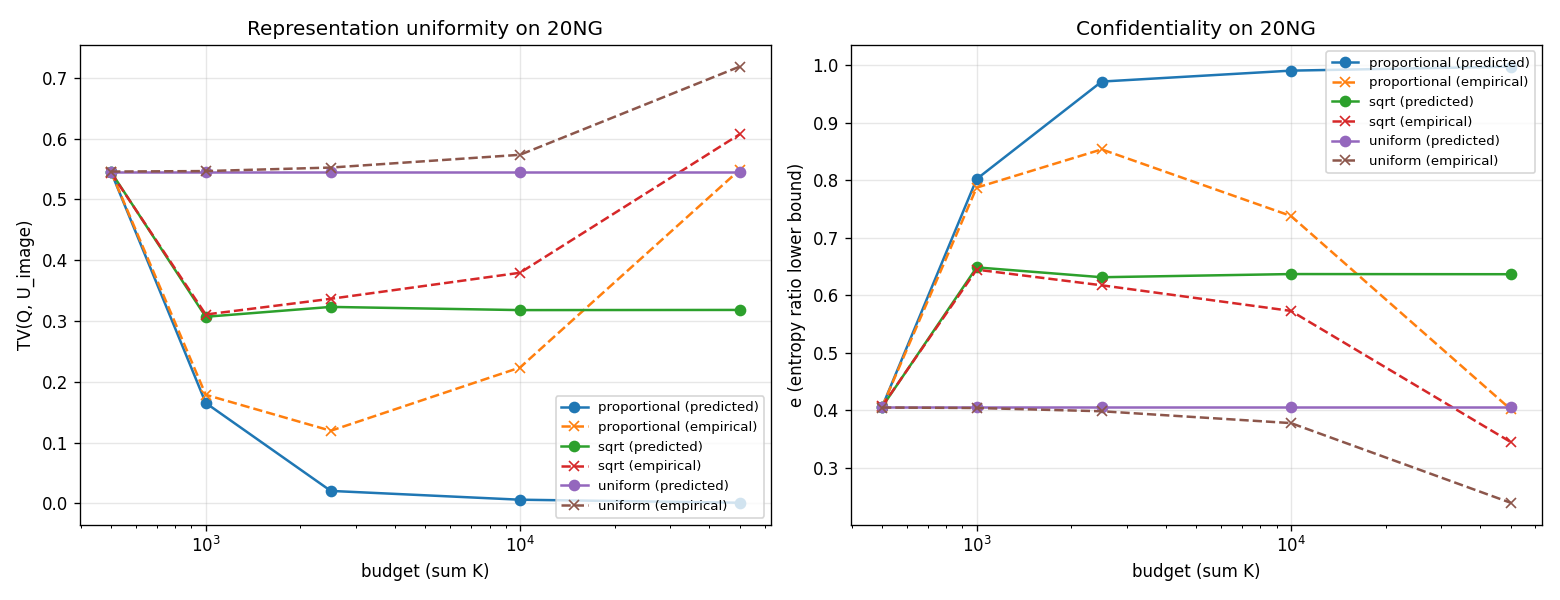
\includegraphics[width=\linewidth]{newsgroups_homophonic}
\caption{Homophonic encoding on the 20 Newsgroups distribution.
Left: representation uniformity $\TV(Q, U_{\mathrm{im}})$ versus
budget for the three allocators (solid: predicted; dashed:
empirical at $N=30{,}000$).  Right: lower bound on the entropy
ratio $e$ from the Fannes-Audenaert inequality.  Proportional
allocation dominates uniform and square-root at every budget.}
\label{fig:newsgroups-homophonic}
\end{figure}

The proportional allocator drops predicted $\TV$ from $0.545$ at
$\sum K = |X|$ (no flexibility) to $0.165$ at $2|X|$ and $0.021$
at $5|X|$, with empirical $e$ rising from $0.40$ to $0.85$.  The
square-root allocator plateaus near $\TV \approx 0.30$ regardless
of budget; it spreads representations too evenly across rare and
common elements.  The uniform allocator does not improve at all,
since its $K$ does not depend on $D$.  At budgets above $20|X|$,
the empirical $\TV$ measurement enters the finite-sample regime
of Appendix~\ref{subsec:finite-sample}: the analytical floor continues
to drop, but $N = 30{,}000$ is no longer enough queries to
resolve it.


\bibliographystyle{IEEEtranN}
\bibliography{refs}

\end{document}
